% Group Id : GC19
% Hadoop add-on API for Advanced Content Based Search \& Retrieval
% BE Computer
% PCCOE
% Members : Kshama Jain, Aditya Kamble, Siddhesh Palande, Rahul Rao


\documentclass[oneside,a4paper,12pt]{report}

\fancypagestyle{plain}{%
  \fancyhf{}
  \fancyfoot[CE]{Pimpri Chinchwad College of Engineering, Department of Computer Engineering 2015}
  \fancyfoot[RE]{\thepage}
}
\pagestyle{fancy}
\fancyhead{}
\renewcommand{\headrulewidth}{0pt}
\footskip = 0.625in
\cfoot{}
\rfoot{}

\usepackage{longtable}
\usepackage{float}
\usepackage{tabu}
\usepackage[]{hyperref}
\usepackage{tikz}
\usetikzlibrary{arrows,shapes,snakes,automata,backgrounds,petri}
\usepackage{tabularx}
\usepackage[nottoc,notlot,notlof,numbib]{tocbibind}
\usepackage[titletoc]{appendix}
\usepackage{titletoc}
\usepackage{float}
\usepackage{subcaption}
\usepackage{multirow}
\usepackage[ruled,vlined]{algorithm2e}

\renewcommand{\appendixname}{Annexure}
\renewcommand{\bibname}{References}
\setcounter{secnumdepth}{5}

\begin{document}

\setlength{\parindent}{0mm}
\begin{center}
{\bfseries SAVITRIBAI PHULE PUNE UNIVERSITY \\}
 \vspace*{1\baselineskip}
{\bfseries A PRELIMINARY PROJECT REPORT ON \\}
 \vspace*{2\baselineskip}
{\bfseries \fontsize{16}{12} \selectfont Hadoop add-on API for Advanced Content Based Search \& Retrieval \\ \vspace*{2\baselineskip}}
{\fontsize{12}{12} \selectfont SUBMITTED TOWARDS THE
 \\PARTIAL FULFILLMENT OF THE REQUIREMENTS OF \\

\vspace*{2\baselineskip}}
{\bfseries \fontsize{14}{12} \selectfont BACHELOR OF ENGINEERING (Computer
Engineering) \\
\vspace*{1\baselineskip}} 

\begin{tabular}{cc}
Kshama Jain  & B120334280 \\
Aditya Kamble  & B120334297 \\
Siddhesh Palande  & B120334356 \\
Rahul Rao  & B120334381 \\[4ex]
\end{tabular}


\textbf{Under The Guidance of} \\[4ex]
Prof. Shailesh Hule \\[4ex]


\includegraphics[width=100pt]{image_pccoelogo.jpg} \\
{\bfseries \fontsize{14}{12} \selectfont DEPARTMENT OF COMPUTER ENGINEERING \\
Pimpri Chinchwad College of Engineering \\
Sector -26, Pradhikaran, Nigdi Pune, Maharashtra 411044
}
\end{center}

\newpage



\begin{figure}[ht]
\centering

\includegraphics[width=100pt]{image_pccoelogo.jpg}
\end{figure}


{\bfseries \fontsize{14}{12} \selectfont \centerline{Pimpri Chinchwad College of Engineering}
\centerline{DEPARTMENT OF COMPUTER ENGINEERING}
\vspace*{1\baselineskip}} 


{\bfseries \fontsize{16}{12} \selectfont \centerline{CERTIFICATE} 
\vspace*{1\baselineskip}} 

\centerline{This is to certify that the Project Entitled}
\vspace*{1\baselineskip} 


{\bfseries \fontsize{14}{12} \selectfont \centerline{Hadoop add-on API for Advanced Content Based Search \& Retrieval}
\vspace*{1\baselineskip}}


\begin{center}
Submitted By \\[4ex]
\begin{tabular}{cc}
Kshama Jain  & B120334280 \\
Aditya Kamble  & B120334297 \\
Siddhesh Palande  & B120334356 \\
Rahul Rao  & B120334381 \\[4ex]
\end{tabular}
\end{center}


is a bonafide work carried out by Students under the supervision of Prof Shweta Koparde and it
is submitted towards the partial fulfillment of the requirement of Bachelor of Engineering (Computer Engineering) Project.\\\\\\

\bgroup
\def\arraystretch{0.7}
\begin{tabular}{c c }
Prof. Shailesh Hule &  \hspace{50 mm} Prof. Dr. K. Rajeswari \\								
Internal Guide   &  \hspace{50 mm} H.O.D \\
Dept. of Computer Engg.  &	\hspace{50 mm}Dept. of Computer Engg.  \\
\end{tabular}
%}

\begin{center}
	%\fontsize{12}{18}\selectfont 
	{
		Dr. A. M. Fulambarkar \\
		Principal\\
		Pimpri Chinchwad College Of Engineering  
	}
\end{center}


Sign of Internal Examiner 
\hspace{40 mm} Sign of External Examiner

% Approval Sheet

\newpage
\begin{center}
	\textbf{PROJECT APPROVAL SHEET}
\end{center}
\begin{center}
Hadoop add-on API for Advanced Content Based Search \& Retrieval
\end{center}

\begin{center}
(Hadoop add-on API for Advanced Content Based Search \& Retrieval)
\end{center}

\begin{center}
Is successfully completed by 
\end{center}

\begin{center}
\begin{tabular}{cc}
	Kshama Jain  & B120334280 \\
	Aditya Kamble  & B120334297 \\
	Siddhesh Palande  & B120334356 \\
	Rahul Rao  & B120334381 \\[4ex]
\end{tabular}
\end{center}

\begin{center}
	at
\end{center} 
\begin{center}
	DEPARTMENT OF COMPUTER ENGINEERING
\end{center}
\begin{center}
	(PIMPRI CHINCHWAD COLLEGE OF ENGINEERING)
\end{center}
\begin{center}
	SAVITRIBAI PHULE PUNE UNIVERSITY,PUNE
\end{center}

\begin{center}
	ACADEMIC YEAR 2015-2016
\end{center}

\vspace*{1\baselineskip}}
\begin{tabular}{c c }
	Prof. Shailesh Hule &  \hspace{50 mm} Prof. Dr. K. Rajeswari \\								
	Internal Guide   &  \hspace{50 mm} H.O.D \\
	Dept. of Computer Engg.  &	\hspace{50 mm}Dept. of Computer Engg.  \\
\end{tabular}


\newpage
\setcounter{page}{0}
\frontmatter
\cfoot{PCCOE, Department of Computer Engineering 2015}
\rfoot{\thepage}
\pagenumbering{Roman}


% Abstract
		
{  \newpage {\bfseries \fontsize{14}{12} \selectfont \centerline{Abstract} 
\vspace*{2\baselineskip}} \setlength{\parindent}{11mm} }
{ \setlength{\parindent}{0mm} }
Unstructured data like doc, pdf, accdb is lengthy to search and filter for desired information. We need to go through every file manually for finding information. It is very time consuming and frustrating. It doesn’t need to be done this way if we can use high computing power to achieve much faster content retrieval.\\\\
We can use features of big data management system like Hadoop to organize unstructured data dynamically and return desired information. Hadoop provides features like Map Reduce, HDFS, HBase to filter data as per user input. Finally we can develop Hadoop Addon for content search and filtering on unstructured data. This addon will be able to provide APIs for different search results and able to download full file, part of files which are actually related to that topic.\\\\
This Addon can be used by other industries and government authorities to use Hadoop for their data retrieval as per their requirement.\\\\
After this addon, we are also planning to add more API features like content retrieval from scanned documents and image based documents.

% Acknowledgement

{  \newpage {\bfseries \fontsize{14}{12} \selectfont \centerline{Acknowledgments} 
\vspace*{2\baselineskip}} \setlength{\parindent}{11mm} }
{ \setlength{\parindent}{0mm} }
\textit{It gives us great pleasure in presenting the preliminary project report 
on {\bfseries \fontsize{12}{12} \selectfont Hadoop add-on API for Advanced Content Based Search \& Retrieval}.}
\vspace*{1.5\baselineskip}

 \textit{We would like to take this opportunity to thank my internal guide
 \textbf{Prof. Shailesh Hule} for giving me all the help and guidance I needed. I am
 really grateful to them for their kind support. Their valuable suggestions were very helpful.} \vspace*{1.5\baselineskip}

 \textit{We am also grateful to \textbf{Prof. Dr. K. Rajeswari}, Head of Computer
 Engineering Department, Pimpri Chinchwad College of Engineering for her indispensable
 support, suggestions.}
\vspace*{1.5\baselineskip}

\textit{In the end our special thanks to \textbf{Prof. Dr. Jayant Umale}, Dean Academics, Pimpri Chinchwad College of Engineering, for his valuable guidance and \textbf{teaching and non teaching staff} for
providing various resources such as  laboratory with all needed software platforms, continuous Internet connection, for Our Project.}
\vspace*{3\baselineskip} \\
\begin{tabular}{p{8.2cm}c}
&Kshama Jain\\
&Aditya Kamble\\
&Siddhesh Palande\\
&Rahul Rao\\
&(B.E. Computer Engg.)
%}
\end{tabular}


\tableofcontents
\listoffigures 
\listoftables


\mainmatter



\titleformat{\chapter}[display]
{\fontsize{16}{15}\filcenter}
{\vspace*{\fill}
 \bfseries\LARGE\MakeUppercase{\chaptertitlename}~\thechapter}
{1pc}
{\bfseries\LARGE\MakeUppercase}
[\thispagestyle{empty}\vspace*{\fill}\newpage]


\setlength{\parindent}{11mm}
\chapter{Synopsis}

\section{Group ID}
GC19

\section{Project Title}
Hadoop add-on API for Advanced Content Based Search \& Retrieval

\section{ Project Option }
Sponsored Project

\section{Internal Guide}
Prof. Shailesh Hule 

\section{ Sponsorship and External Guide} 
Mr. Atul Shimpi ( Persistent Systems ) 


\section{Technical Keywords (As per ACM Keywords)}
\begin{itemize}
\item Hadoop
\item HDFS
\item MapReduce
\item HBase
\item Content Based System
\end{itemize}



\section{Problem Statement}
\label{sec:problem}
Hadoop add-on API for Advanced Content Based Search \& Retrieval

\section{Abstract}

Unstructured data like doc, pdf, accdb is lengthy to search and filter for desired information. We need to go through every file manually for finding information. It is very time consuming and frustrating. It doesn’t need to be done this way if we can use high computing power to achieve much faster content retrieval.\\\\
We can use features of big data management system like Hadoop to organize unstructured data dynamically and return desired information. Hadoop provides features like Map Reduce, HDFS, HBase to filter data as per user input. Finally we can develop Hadoop Addon for content search and filtering on unstructured data. This addon will be able to provide APIs for different search results and able to download full file, part of files which are actually related to that topic.\\\\
This Addon can be used by other industries and government authorities to use Hadoop for their data retrieval as per their requirement.\\\\
After this addon, we are also planning to add more API features like content retrieval from scanned documents and image based documents.

\section{Goals and Objectives}
\textbf{Goals:} \\
Current Systems Focus on Search by Title,Author,etc which Is time consuming and finding relevant content from those documents is tedious task. So there is a need of such a system which shall find the relevant contents to the end user \\

\noindent \textbf{Objective:} \\
To find the relevant content from the huge number of PDF files present on Hadoop Distributed File System \\

	
\section{Relevant mathematics associated with the Project}
\noindent
S = \{s,e,x,y,DD,NDD,Mem-shared\} \\\\
s = start state : Taking input from the user as search query \\
e = End State : return the output to the user in the form text based content \\\\
x = Input : Search Query \\
y = Output : Text Based Result \\\\
DD = Deterministic Data \\
1) Number of PDF Files \\
2) Keyword Tokenisation and Filteration \\
3) Number of DataNodes 
4) Search Progress 
5) Number of Results Obtained \\\\
NDD = Non Deterministic Data \\
1) Failure of Cluster Nodes \\
2) Communication Failure  \\\\
Mem-Shared = Storage Space 
1) HDFS will be distributed among a number of nodes in Hadoop Cluster and will share common FileSystem which will be managed by Hadoop \\


\section{Names of Conferences / Journals where papers can be published}
\begin{itemize}
\item IOSR - International Organization of Scientific Research
\item ICCUBEA - International Conference on Computing, Communication, Control And Automation
\end{itemize} 


\section{Review of Conference/Journal Papers supporting Project idea}
\label{sec:survey}
\begin{enumerate}
\item \textbf{Paper Title } : Hadoop add-on API for Advanced Content Based Search \& Retrieval 
\item \textbf{Name of the Conference/Journal where paper submitted } : IOSR - International Organization of Scientific Research
\item \textbf{Paper accepted/rejected } : Accepted
\item \textbf{Review comments by reviewer} : The independent review upon your research article titled "Hadoop add-on API for Advanced Content Based Search \& Retrieval" has been provided by the concerned referees. The referees have suggested Accepted your paper in IOSR Journals.
	\begin{enumerate}
		\item Quality of Manuscript is good.
		\item Consolidated Decision: Accepted for publication 
	\end{enumerate}
	
\end{enumerate}

{\tabulinesep=2mm
   \begin{longtabu} { |p{3.5cm} | p{3.5cm} | p{4cm }| p{2.5cm }|}
       \hline

\textbf{Title} & \textbf{Keyword} & \textbf{Content} & \textbf{Author}\\ \hline
Context based Indexing in Search Engines using Ontology &
Context, indexing, posting list, context repository, ontology repository &
Indexing in search engines has been an active area of current researches. The main aim of search engines is to provide most relevant documents to the users in minimum possible time. So granting efficient and fast accesses to the index is a major issue for performances of Web Search Engines &
Parul Gupta, Dr. A.K.Sharma \\ \hline

Hadoop-HBase for Large- Scale  Data (2011) &
large-scale  data;  distributed  storage;  Hadoop; HDFS; Map Reduce; HBase; noSQL database &
The  paper  aims  at evaluating the performance of random reads and random writes of data storage location information to HBase and retrieving and storing  data  in  HDFS  respectively. &
Mehul Nalin Vora \\ \hline

High Performance and Fault Tolerant Distributed File System for Big Data Storage and Processing using Hadoop(2014) &
Big data; Analytics; Hadoop; Hadoop Distributed File System (HDFS); Hype cycle; MapReduce; Replication; Faulttolerance; Unstructured data &
In this paper they have highlighted the evolution and rise of big data  and discussed how HDFS produces multiple replicas of data. &
E.Sivaraman, Dr.R. Manickachezian \\ \hline

Handling Big Data Efficiently by using Map Reduce Technique(2014) &
Data Mining; Clustering; DBMS; Parallel processing; Hadoop; MapReduce. &
 In this paper, They discussed work around MapReduce, its advantages, disadvantages and how it can be used in integration with other technology. &
Seema Maitrey, C.K. Jha \\ \hline

The Dawn of Big Data - Hbase &
HBase, Hadoop Distributed File System (HDFS), HBase column oriented table. &
This paper includes the step by step introduction to the HBase,IdentifY differences between apache HBase and a traditional RDBMS. &
Vijayalakshmi Bhupathirajul, Ravi Prasad Ravud \\ \hline
      
   \end{longtabu}
}

\section{Plan of Project Execution}
\begin{table}[!htbp]
\begin{center}
\def\arraystretch{1.5}
  \begin{tabular}{| c | c | c | c |}
       \hline

	\textbf{Activity} & \textbf{Weeks to Spend} & \textbf{Deliverables} & \textbf{Priority}\\ \hline
	Analysis of Existing System & 2 weeks & - & Normal \\ \hline
	Requirement Gathering & 2 weeks & Requirements & Normal \\ \hline 
	Literature Survey & 3 Week & - & Normal \\ \hline
	Designing and Planning & 5 weeks & Modules & High \\ \hline
	Implementation & 10 weeks & API & High \\ \hline
	Testing & 3 weeks & Test Report & High \\ \hline
	Documentation & 4 week & Project Report & Normal \\ \hline
\end{tabular}
 \caption { Plan of Project Execution }
 \label{tab:hreq}
\end{center}

\end{table}



\chapter{Technical Keywords}
\section{Area of Project}
\begin{itemize}
\item Big data and Hadoop
\item Content Based Search and retrieval
\end{itemize}

\section{Technical Keywords}
\begin{enumerate}
\item Hadoop: Hadoop is an open-source framework that allows to store and process big data in a distributed environment across clusters of computers using simple programming models. 
\begin{itemize}
\item Distributed
\item Scalable
\item Fault-tolerant
\item Open source
\end{itemize}

\item HDFS:
\begin{itemize}
\item HDFS, the Hadoop Distributed File System, is responsible for storing data on the cluster.
\item Data is split into blocks and distributed across multiple nodes in the cluster. 
\item HDFS is a Java-based file system that provides scalable and reliable data storage, and it was designed to span large clusters of commodity servers.
\end{itemize}


\item MapReduce
\begin{itemize}
\item MapReduce is the system used to process data in the Hadoop Cluster.
\item Consist of to phases:Map and the Reduce
\item Each map task operates on discrete portion of the overall dataset
\item After all Maps are compete, the mapReduce system distributes the intermediate data to nodes which perform the Reduce phase
\end{itemize}

\item HBase
\begin{itemize}
\item HBase is an open source, non-relational, distributed database 
\item The data is partitioned based on the RowKeys into Regions.
\item Each Region contains a range of RowKeys based on their binary order.
\item A RegionServer can contain several Regions.
\end{itemize}

\item Content based:
\begin{itemize}
\item Using information manually entered or included in the table design, such as titles, descriptive keywords from a limited vocabulary, and predetermined classification schemes. The primary benefit of using content-based retrieval is reduced time and effort required to obtain image-based information.
\end{itemize}

\end{enumerate}

			

\chapter{Introduction}
\section{Project Idea}
Basic project idea is to reduce manual efforts for content based searching in large set of documents using Hadoop Big Data Management framework to automate content based searching and retrieving the relevant content. 


\section{Motivation of the Project}  
\begin{itemize}
\item Taks like assignment completion, taking notes from text books and reference books on particular topic, topics for presentation need deep reading and need to go through every document manually just to find relevant content on given topic.
\item Currently present systems are only searching based on document title, author, size, and time but not on content. So to do content based search on big data documents and large text data Haddop framework can be used.
\item So using Hadoop Big Data management framework consist of HDFS, MapReduce, and HBase, we are developing content based search on PDF documents to solve real life problem. So this is basic motivation for the project.
\end{itemize}

\newpage

\section{Literature Survey}
{\tabulinesep=2mm
   \begin{longtabu} { |p{3.5cm} | p{3.5cm} | p{4cm }| p{2.5cm }|}
       \hline

\textbf{Title} & \textbf{Keyword} & \textbf{Content} & \textbf{Author}\\ \hline
Context based Indexing in Search Engines using Ontology &
Context, indexing, posting list, context repository, ontology repository &
Indexing in search engines has been an active area of current researches. The main aim of search engines is to provide most relevant documents to the users in minimum possible time. So granting efficient and fast accesses to the index is a major issue for performances of Web Search Engines &
Parul Gupta, Dr. A.K.Sharma \\ \hline

Hadoop-HBase for Large- Scale  Data (2011) &
large-scale  data;  distributed  storage;  Hadoop; HDFS; Map Reduce; HBase; noSQL database &
The  paper  aims  at evaluating the performance of random reads and random writes of data storage location information to HBase and retrieving and storing  data  in  HDFS  respectively. &
Mehul Nalin Vora \\ \hline

High Performance and Fault Tolerant Distributed File System for Big Data Storage and Processing using Hadoop(2014) &
Big data; Analytics; Hadoop; Hadoop Distributed File System (HDFS); Hype cycle; MapReduce; Replication; Faulttolerance; Unstructured data &
In this paper they have highlighted the evolution and rise of big data  and discussed how HDFS produces multiple replicas of data. &
E.Sivaraman, Dr.R. Manickachezian \\ \hline

Handling Big Data Efficiently by using Map Reduce Technique(2014) &
Data Mining; Clustering; DBMS; Parallel processing; Hadoop; MapReduce. &
 In this paper, They discussed work around MapReduce, its advantages, disadvantages and how it can be used in integration with other technology. &
Seema Maitrey, C.K. Jha \\ \hline

The Dawn of Big Data - Hbase &
HBase, Hadoop Distributed File System (HDFS), HBase column oriented table. &
This paper includes the step by step introduction to the HBase,IdentifY differences between apache HBase and a traditional RDBMS. &
Vijayalakshmi Bhupathirajul, Ravi Prasad Ravud \\ \hline
      
   \end{longtabu}
}


\chapter{Problem Definition and scope}
\section{Problem Statement}
Hadoop add-on API for Advanced Content Based Search \& Retrieval

\subsection{Goals and objectives}  
\noindent \textbf{Goals:} \\
Current Systems Focus on Search by Title,Author,etc which Is time consuming and finding relevant content from those documents is tedious task. So there is a need of such a system which shall find the relevant contents to the end user \\

\noindent \textbf{Objective:} \\
To find the relevant content from the huge number of PDF files present on Hadoop Distributed File System \\


 \subsection{Statement of scope} 
This system shall retrieve the required contents of files which are in an unstructured format containing huge amount of Data like e-books in a digital library where the number of books are present in thousands. The scope here is initially limited to PDF files which may be expanded to other unstructured formats like ePUB, mobi.\\\\
The input is provided to the system API in the form of search query which will be firstly filtered to find the important expression as a query to the API which will return the important content to the user in the form of paragraph or text highlighted using the power of distributed computing. \\\\
The particular page or the Entire book itself can be downloaded by the Library users if the content is satisfied else the search continues for finding relevant content

\section{Software context} 
The end product of this project is the API for the distributed system having hadoop distributed system which would have enhanced abilities in searching the relevant contents inside big data of documents in a very rapid manner by completely harnessing the power of distributed computing and searching algorithms.This API shall be provided as an AddOn feature on top of Hadoop specially for content based retrieval purposes which would mainly deal with unstructured big data like PDF files.

\section{Major Constraints}
\begin{enumerate}
\item The first constraint is the that API used on a standalone system would not provide good performance required for content based retrieval system developed by the developer.
\item A pseudo distributed system deployed using different number of virtual machines would almost provide the similar performance as that of standalone systems depending on the number of virtual machine instances running simultaneously and the amount of memory allocated to each instance.Here care must be taken that guest nodes should not become a bottleneck to the hosted master node.
\item The best and suggested recomendation is that the API should be used and deployed on a fully-distributed system of nodes each connected to each other having independent memory ,disk and processor which will perform the best and provide expected results.
\end{enumerate}

\section{Methodologies of Problem solving and efficiency issues}
\begin{enumerate}
\item Single Mode
When a cluster with only a single node is used for implementing the content based retrieval system,slower performance is expected due to the less amount of memory and processing power.

\item Pseudo Distributed Mode
When a system is implemented either with number of virtual machines the different daemons as different process then the system is expected to perform better 

\item Fully Distributed Mode
When a cluster has number of physical nodes and hadoop daemons as different java processes with greater than 10 or more nodes in a single rack then the expected results are expected to be more better due to the presence of large storage and processing power.
\end{enumerate}

\section{Scenario in which multi-core, Embedded and Distributed Computing used}
The trends are nowadays shifting from standalone single node applications to distributed applications where in Java Frameworks like Hadoop help the applications to utlize the power of distributed computing wherein each and every node is assigned a task and the result is obtained to the master node which assigns the tasks to the slave nodes.

\section{Outcome}
\begin{enumerate}
\item The system is expected to provide the content based on the keywords entered in the form of keywords and the output shall be in the form of any of the following formats:
\item Entire Document
\item Content and the required paragraphs surrounding it
\item Only Paragraph itself 
\item Only Particular Page itself
and many such options shall be provided in the API.
\end{enumerate}

\section{Applications}
\begin{itemize}
\item Content based search and retrieval on
\begin{enumerate}
\item Digital library books 
\item IEEE Papers
\item Private Authorities
\item Government Authorities
\item Unstructured text files
\end{enumerate}

\item This API can be used to develop above functionality on platforms like
\begin{enumerate}
\item Web Application
\item Android Application
\item Standalone Application
\item Command Line Interface Application
\end{enumerate}

\end{itemize}

\section{Hardware Resources Required}
\begin{itemize}	
\item Memory require for Hadoop installation and HBase and Map Reduce components.
\item API requires minimum 100 MB space as it contains core components for content based retrieval
\item 4 GB Primary Memory / RAM
\item Intel i3/i5/i7 64bit or AMD Processors
\item SSH Authentication to communicate with Namenode and Datanodes
\end{itemize}


\section{Software Resources Required}
\begin{itemize}
\item Any Open Source Linux Distribution.(Ubuntu Server version 14.04.2 Preferred)
\item OPENSSH installed on each machine with public key of each node in authorized\_keys directory along with the localhost.
\item JDK Version 1.7 or above
\item JAVA\_HOME to be appended in the \$PATH environment variable
\item Hostname to be initialized for each node in the /etc/hosts file having a masternode (namenode), secondary namenode and various slave nodes to be added.
\item \$HADOOP\_HOME environment variable path to added in the ~/.bashrc 
\item Following Files to be configured in \$HADOOP\_HOME/etc/hadoop directory
\end{itemize}

\chapter{Project Plan}

\section{Project Estimates}
             
\subsection{Reconciled Estimates}
Reconciliation is the method of bringing together all of the data and analyses into one final estimate of value. Hence following is the total data which we have reconciled and given approx metric of all the factors. \\

\subsubsection{Cost Estimate}
The costing feasibility of the project can be estimated using current estimation models such as lines of code, which allows us to estimate cost as a function of size. Thus, this also allows us to estimate and analyze the feasibility of competition of the system in the given time frame. This allows us to have a realistic estimate as well as a continuous evaluative perspective of the progress of the project. 

\subsubsection{Time Estimates}
Our product will take 8 months to be completed before it is useful. Our product timetable is reasonable as it takes 3 months to be study requirements, to develop analysis model and to develop a design and 5 months to implement a product with the given specification. A project deadline is month end of March and it is reasonable, mandatory as well.


\subsection{Project Resources}
\textbf{ \\ Hardware Resources}
\begin{itemize}
\item There shall be N number of nodes each having the following hardware configuration in a fully distributed system connected environment together in a wired manner using Ethernet interface.
\item Intel i3/i5/i7 processor
\item Ethernet Interface on NIC
\item Virtualization of upto 2 or 3 nodes on a single machine for testing purposes
\item 2 or 4 GB RAM (and upto 512 MB for each node for pseudo disrtibuted) \\[3ex]
\end{itemize}

\noindent \textbf{Software Resources}
\begin{itemize}
\item Any Open Source Linux Distribution.(Ubuntu Server version 14.04.2 Preferred)
\item OPENSSH installed on each machine with public key of each node in authorized\_keys directory along with the localhost.
\item JDK Version 1.7 or above
\item JAVA\_HOME to be appended in the \$PATH environment variable
\item Hostname to be initialized for each node in the /etc/hosts file having a masternode (namenode), secondary namenode and various slave nodes to be added.
\item \$HADOOP\_HOME environment variable path to added in the ~/.bashrc 
\item Following Files to be configured in \$HADOOP\_HOME/etc/hadoop directory

	\begin{enumerate}
	\item core-site.xml
	\item hadoop-env.sh
	\item yarn-site.xml
	\item mapred-site.xml
	\item master
	\item slave
	\end{enumerate}

\item Master node with Ubuntu Workstation version preferred for supporting Eclipse IDE with Hadoop plugin for development and Server having Ubuntu Server version Preferred. \\[3ex]
\end{itemize}

\noindent \textbf{Tools}
\begin{itemize}
\item Eclipse IDE
\item Hadoop Eclipse Plugin
\item Java 1.7
\item Hadoop Java Libraries.
\end{itemize}

\section{Project Schedule}  
\subsection{Project task set}  
Major Tasks in the Project stages are: 
\begin{itemize}
\item Create distributed system with Hadoop namenodes and datanodes
\item Develop API methods for extracting keywords from input query
\item Test API methods for finding keywords from input query
\item Develop API methods to perform keyword search on HDFS data using Map Reduce operations
\item Test API methods to perform keyword search on HDFS data using Map Reduce operations
\item Design database schema for indexing each and every document in HDFS
\item Schema validation for HBase indexing database
\item Develop background service for indexing newly added data to HBase database automatically
\item Test background service for indexing newly added data to HBase database is working automatically or not
\item Integrating all modules
\item Integration testing
\end{itemize}

\subsection{Task network}
\begin{center}
	\begin{figure}[!htbp]
		\centering
		\fbox{
\includegraphics[width=\textwidth]{task_network}}
	  \caption{Task network}
	  \label{fig:usecase}
	\end{figure}
\end{center}
  
\pagebreak
\subsection{Timeline Chart}  
\begin{center}
	\begin{figure}[!htbp]
		\centering
		\fbox{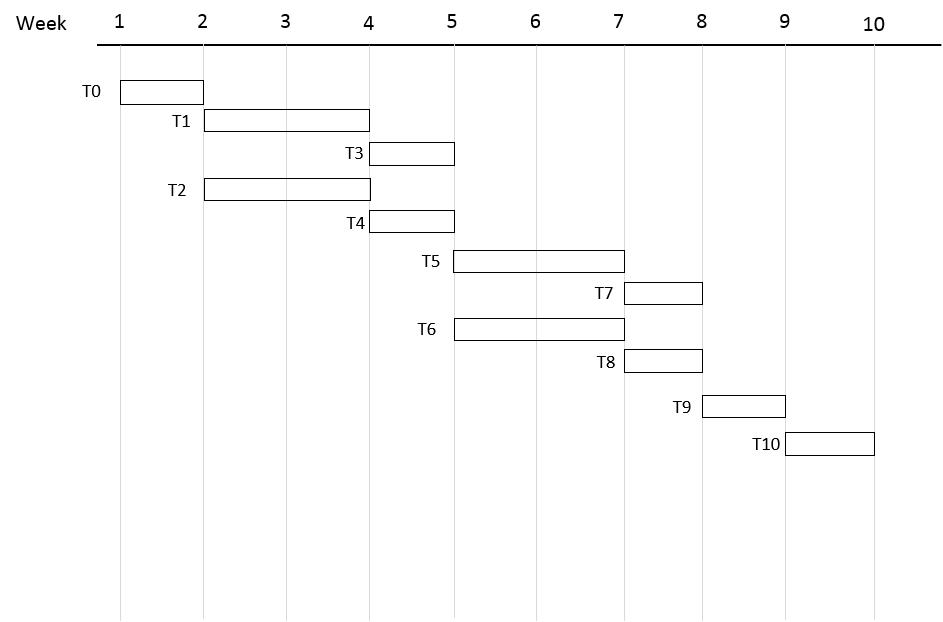
\includegraphics[width=\textwidth]{timeline_chart}}
	  \caption{Project Planning Chart 1}
	  \label{fig:usecase}
	\end{figure}
\end{center}
 
\section{Team Organization}

\subsection{Team structure}
For this project team is of 4 developers. 
\begin{table}[!htbp]
\begin{center}
\def\arraystretch{1.5}
  \begin{tabular}{| c | c |}
       \hline
       
Team Member & Roles \\ \hline
Kshama Jain & Literature Survey and Solution Analysis \\ \hline
Aditya Kamble & Software API Development and Testing \\ \hline
Rahul Rao & System Management and API Development \\ \hline
Siddhesh Palande & Integration and Testing \\ \hline
       
\end{tabular}
 \caption { Team Structure }
 \label{tab:hreq}
\end{center}

\end{table}

\subsection{Management reporting and communication}
The communication and reporting of work is done on weekly basis depending upon the time which is around 4hrs for a week and since they are sharing the same premises the communication is also excellent.
 
\chapter{Software requirement specification  (SRS is to be prepared using relevant mathematics derived and software engg. Indicators in Annexure A and B)}

\section{Introduction}
Unstructured data like doc, pdf, accdb is lengthy to search and filter for desired information. We need to go through every file manually for finding information. It is very time consuming and frustrating. It doesn’t need to be done this way if we can use high computing power to achieve much faster content retrieval.\\\\
We can use features of big data management system like Hadoop to organize unstructured data dynamically and return desired information. Hadoop provides features like Map Reduce, HDFS, HBase to filter data as per user input. Finally we can develop Hadoop Addon for content search and filtering on unstructured data. This addon will be able to provide APIs for different search results and able to download full file, part of files which are actually related to that topic.\\\\
This Addon can be used by other industries and government authorities to use Hadoop for their data retrieval as per their requirement.\\\\
After this addon, we are also planning to add more API features like content retrieval from scanned documents and image based documents

\subsection{Purpose and Scope of Document}
The Software Requirement Specification or SRS is a document which provides the stakeholders in the project about the overview of the project. Every project or software has a document which tell about the software, the requirement of the software such as hardware requirement, software requirement, functional requirement, non functional requirement, security requirement and other requirement. It also provides the information about the flow of the software, use cases. \\

The SRS document will help the developers to understand the user requirement and the specifications and architecture of the software. In future, if any changes are to be made in the software, the SRS provides the developer the details of the software project which will help the developer to understand the make appropriate changes to the software. 


\subsection{Overview of responsibilities of Developer}
\begin{enumerate}
\item The developer should have the knowledge of Hadoop.
\item The developer should have the knowledge of Java.
\item The developer should have the knowledge of HBase.
\item The developer should have the knowledge of Testing.
\end{enumerate}


\section{Usage Scenario}
This section provides various usage scenarios for the system to be developed.
 
 \subsection{User profiles}  
There will be number of users who will use the same application which will be provided by the developer. As the user search for query in the HDFS of Distributed Hadoop System, system will return the result with expected outcome. 

\subsection{Use-cases}
All use-cases for the software are presented.

{\tabulinesep=2mm
   \begin{longtabu} { |p{2.5cm} | p{2.5cm} | p{2.5cm }| p{2.5cm }| p{2.5cm }|}
       \hline

\textbf{Sr No} & \textbf{Use Case } & \textbf{Actor} & \textbf{Description} & \textbf{Goals} \\ \hline

1 & Use case 1 & User & Add Document & User add document to HDFS system using API  Insert user added document to HDFS and scan for keywords to store in metadata.
\\ \hline
2 & Use case 2 & Administrator & Setup Hadoop cluster. & Hadoop cluster will work with our addon API for content based retrieval. \\ \hline

   \end{longtabu}
}


\subsection{Use Case View}
Use Case Diagram. Example is given below
\begin{center}
	\begin{figure}[H]
		\centering
		\fbox{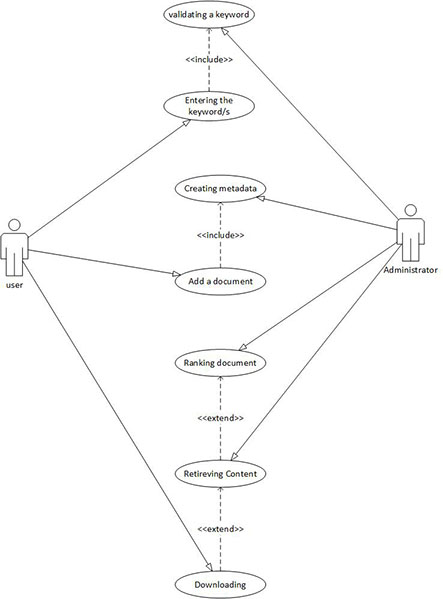
\includegraphics[width=\textwidth]{use_case_diagram}}
	  \caption{Use case diagram}
	  \label{fig:usecase}
	\end{figure}
\end{center}  

\section{Data Model and Description}  
\subsection{Data Description}
In this project we are searching and retrieving information from data inside HDFS. Hadoop Map Reduce operations will be used to perform key value pair generation and depend upon result information is searched.\\\\
Here, data is documents in PDF ( Portable Document Format ) format. These documents are stored on HDFS - Hadoop Distributed File System. These documents are considered as raw data. These documents can have properties like
\begin{itemize}
\item Name
\item Size
\item Date
\item Author
\end{itemize}
Document meta data is also maintain in HBase distributed database. It has attributes like
\begin{itemize}
\item Content Keywords
\item Index Keyword
\item Document Keywords
\item Keywords Frequency
\end{itemize}
This information will be useful to filter documents before performing content based  searching operations.



\subsection{Data objects and Relationships}
\begin{center}
	\begin{figure}[H]
		\centering
		\fbox{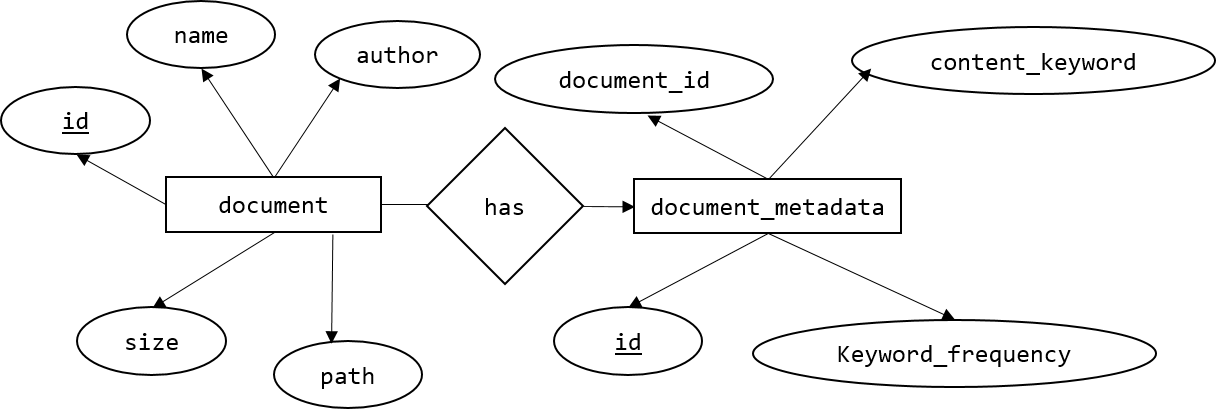
\includegraphics[width=\textwidth]{data_model}}
	  \caption{Data Model}
	  \label{fig:data-model}
	\end{figure}
\end{center}  
 
 
\section{Functional Model and Description}  
A description of each major software function, along with data flow (structured analysis) or class hierarchy (Analysis Class diagram with class description for object oriented system) is presented. 

\subsection{Data Flow Diagram}  
\begin{center}
	\begin{figure}[H]
		\centering
		\fbox{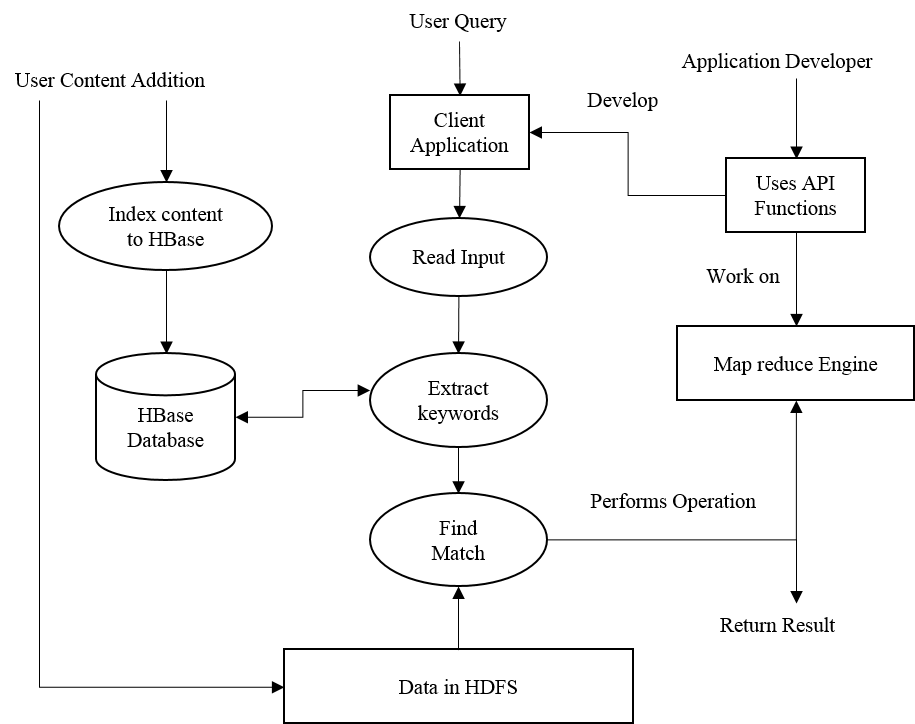
\includegraphics[width=\textwidth]{data_flow}}
	  \caption{Data Flow Diagram}
	  \label{fig:data-flow}
	\end{figure}
\end{center} 
 
 
\subsection{Activity Diagram:}
\begin{center}
	\begin{figure}[H]
		\centering
		\fbox{
\includegraphics[height=430pt]{activity_diagram}}
	  \caption{Activity diagram}
	  \label{fig:act-dig}
	\end{figure}
\end{center}  

\subsection{Non Functional Requirements:}
\textbf{Performance Requirements} \\ \\
Memory Requirements:
\begin{itemize}	
\item Memory require for Hadoop installation and HBase and Map Reduce components.
\item API requires minimum 100 MB space as it contains core components for content based retrieval
\item 4 GB Primary Memory / RAM
\end{itemize}

Speed Requirements:
\begin{itemize}
\item Intel i3/i5/i7 64bit or AMD Processors
\end{itemize}

\noindent \textbf{Security Requirements}
\begin{itemize}
\item SSH Authentication to communicate with Namenode and Datanodes
\end{itemize}

\noindent \textbf{Software Quality Attributes}
Software Quality can be defined as “the conformance to explicitly stated functional and performance requirements, explicitly documented development standards, and implicit characteristics that are expected of all professionally developed software”.\\
	
\noindent \textbf{Software Quality Attributes are}

\begin{enumerate}
\item \textbf{Functionality}
This is an ability by which the software satisfies the needs of the software denoted by suitability, accuracy, interoperability, compliance and security.

\item \textbf{Reliability}
Due to wired connectivity, reliability can be guaranteed.

\item \textbf{Availability}
The system should be available during their respected hours.

\item \textbf{Usability}
This ability indicates that the usefulness of the software.

\item \textbf{Efficiency}
This indicates the measure of computing resources and time required by the program to perform.

\item \textbf{Maintainability}
The ability required to locate or fix bugs in software. There should be facility to add or delete or update documents.

\item \textbf{Portability}
The software works properly even if the environment gets changed (i.e. change in hardware or software).

\item \textbf{Reusability}
With new versions of Hadoop this API can be improved using new features of Hadoop
\end{enumerate}





\subsection{State Diagram:}	
A state diagram is a type of diagram used in computer science and related fields to describe the behavior of systems. State diagrams require that the system described is composed of a finite number of states; sometimes, this is indeed the case, while at other times this is a reasonable abstraction. Many forms of state diagrams exist, which differ slightly and have different semantics


\begin{center}
	\begin{figure}[H]
		\centering
		\fbox{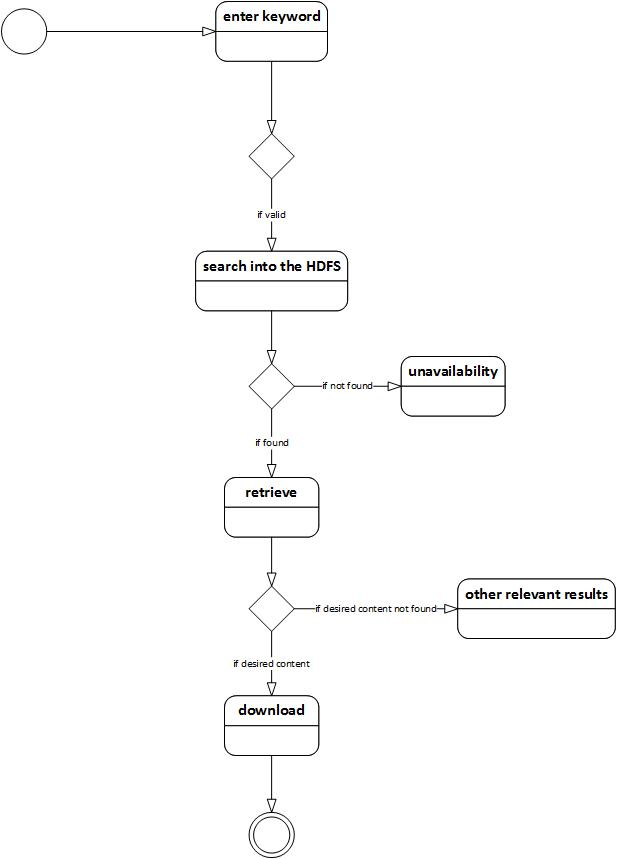
\includegraphics[width=230pt]{statemachine_diagram}}
	  \caption{State transition diagram}
	  \label{fig:state-dig}
	\end{figure}
\end{center} 
 
 \subsection{Design Constraints}	
The primary design constraint is the distributed platform. Since the application is designated for distributed systems. Creating a Application Programming  Interface which is both effective and easily usable will pose a difficult challenge. Other constraints such as limited memory and processing power are also worth considering.

 \subsection{Software Interface Description}	 
\begin{itemize}
\item Any Open Source Linux Distribution.(Ubuntu Server version 14.04.2 Preferred)
\item OPENSSH installed on each machine with public key of each node in authorized\_keys directory along with the localhost.
\item JDK Version 1.7 or above
\item JAVA\_HOME to be appended in the \$PATH environment variable
\item Hostname to be initialized for each node in the /etc/hosts file having a masternode (namenode), secondary namenode and various slave nodes to be added.
\item \$HADOOP\_HOME environment variable path to added in the ~/.bashrc 
\item Following Files to be configured in \$HADOOP\_HOME/etc/hadoop directory

	\begin{enumerate}
	\item core-site.xml
	\item hadoop-env.sh
	\item yarn-site.xml
	\item mapred-site.xml
	\item master
	\item slave
	\end{enumerate}

\item Master node with Ubuntu Workstation version preferred for supporting Eclipse IDE with Hadoop plugin for development and Server having Ubuntu Server version Preferred.
\end{itemize}



\chapter{Detailed Design Document using Appendix A and B}
 \section{Introduction}  
This document specifies the design that is used to solve the problem of Product.  

\section{Architectural Design}  
 
  \begin{center}
	\begin{figure}[!htbp]
		\centering
		\fbox{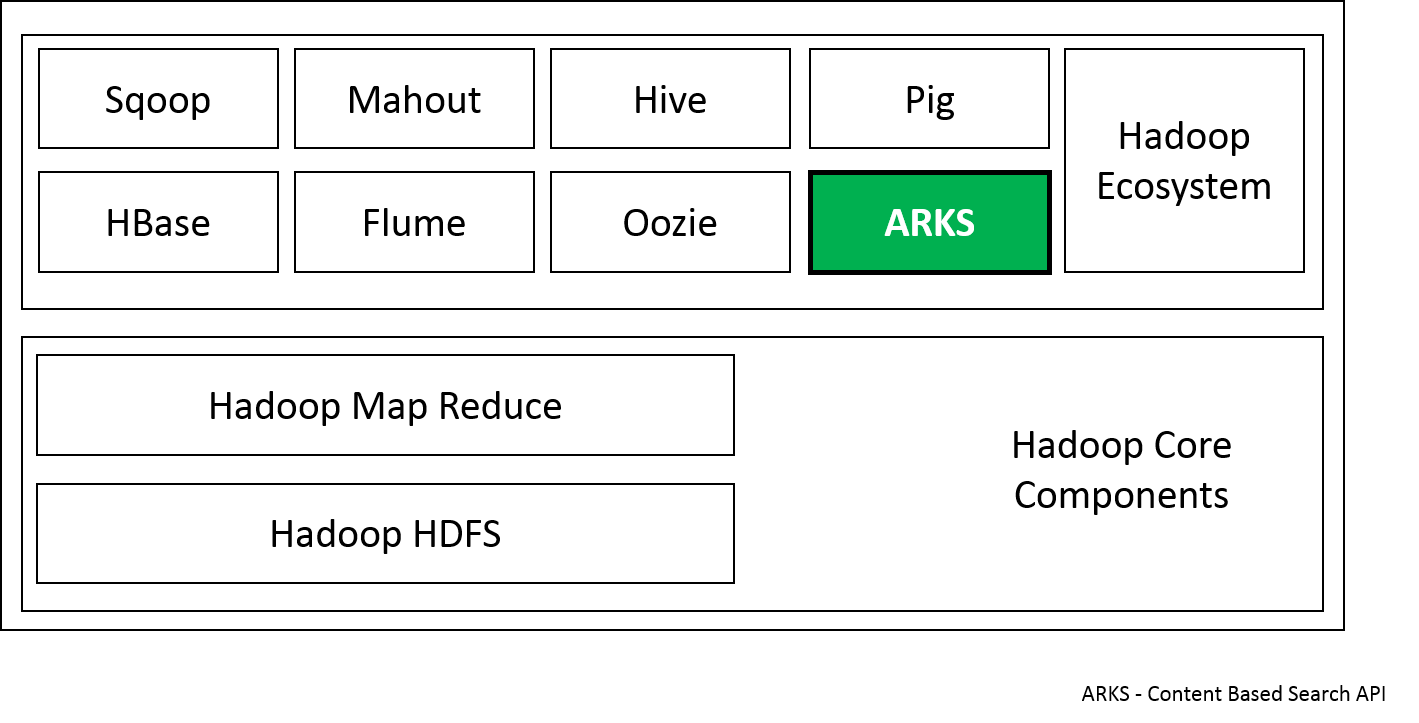
\includegraphics[width=\textwidth]{cbsa-layer-architecture}}
	  \caption{Architecture diagram}
	  \label{fig:arch-dig}
	\end{figure}
\end{center} 


\section{Data design (using Appendices A and B)}   
This section includes a description of all data structures including internal, global, and temporary data structures, database design (tables), file formats

\subsection{Internal software data structure}
We are using HashMap as internal datastructure since MapReduce uses it. \\
A HashMap is an object that maps keys to values. A map cannot contain duplicate keys: Each key can map to at most one value. It models the mathematical function abstraction. The Map interface includes methods for basic operations (such as put, get, remove, containsKey, containsValue, size, and empty), bulk operations (such as putAll and clear), and collection views (such as keySet, entrySet, and values). \\
Creating Hashmap datastructure: Map<String, Integer> m = new HashMap<String, Integer>(); \\ \\
     
The second argument is a conditional expression that has the effect of setting the frequency to one if the word has never been seen before or one more than its current value if the word has already been seen. Try running this program with the command:
java Freq if it is to be it is up to me to delegate
The program yields the following output.
8 distinct words: {to=3, delegate=1, be=1, it=2, up=1, if=1, me=1, is=2}
Suppose we prefer to see the frequency table in alphabetical order. All you have to do is change the implementation type of the Map from HashMap to TreeMap. Making this four-character change causes the program to generate the following output from the same command line.
8 distinct words: {be=1, delegate=1, if=1, is=2, it=2, me=1, to=3, up=1}
Similarly, we make the program print the frequency table in the order the words first appear on the command line simply by changing the implementation type of the map to LinkedHashMap. Doing so results in the following output.
8 distinct words: {if=1, it=2, is=2, to=3, be=1, up=1, me=1, delegate=1



\subsection{Global data structure}
We are using Set interface as Global datastructure.\\
	A Set is a Collection that cannot contain duplicate elements. It models the mathematical set abstraction. The Set interface contains only methods inherited from Collection and adds the restriction that duplicate elements are prohibited. Set also adds a stronger contract on the behavior of the equals and hashCode operations, allowing Set instances to be compared meaningfully even if their implementation types differ. Two Set instances are equal if they contain the same elements.\\
The Java platform contains three general-purpose Set implementations: HashSet, TreeSet, and LinkedHashSet. HashSet, which stores its elements in a hash table, is the best-performing implementation; however it makes no guarantees concerning the order of iteration. TreeSet, which stores its elements in a red-black tree, orders its elements based on their values; it is substantially slower than HashSet. LinkedHashSet, which is implemented as a hash table with a linked list running through it, orders its elements based on the order in which they were inserted into the set (insertion-order). LinkedHashSet spares its clients from the unspecified, generally chaotic ordering provided by HashSet at a cost that is only slightly higher.


\subsection{Temporary data structure}
Arrays as temporary datastructures: \\
An array is an object of reference type which contains a fixed number of components of the same type; the length of an array is immutable. Creating an instance of an array requires knowledge of the length and component type. Each component may be a primitive type (e.g. byte, int, or double), a reference type (e.g. String, Object, or java.nio.CharBuffer), or an array. Multi-dimensional arrays are really just arrays which contain components of array type. \\
Arrays are implemented in the Java virtual machine. The only methods on arrays are those inherited from Object. The length of an array is not part of its type; arrays have a length field which is accessible via java.lang.reflect.Array.getLength().
Reflection provides methods for accessing array types and array component types, creating new arrays, and retrieving and setting array component values.

\subsection{Database description}
\begin{table}[!htbp]
\begin{center}
\def\arraystretch{1.5}
  \begin{tabular}{| c | c |}
       \hline
       
Fields & Type \\ \hline
id & int \\ \hline
name & varchar(50) \\ \hline
author & varchar(50) \\ \hline
size & int \\ \hline
path & string \\ \hline
       
\end{tabular}
 \caption { Table - Document  }
 \label{tab:hreq}
\end{center}

\end{table}

\begin{table}[!htbp]
\begin{center}
\def\arraystretch{1.5}
  \begin{tabular}{| c | c |}
       \hline
       
Fields & Type \\ \hline
document\_id & int \\ \hline
content\_keyword & varchar(50) \\ \hline
index\_keyword & varchar(50) \\ \hline
keyword\_frequency & varchar(50) \\ \hline
       
\end{tabular}
 \caption { Table - Document Metadata  }
 \label{tab:hreq}
\end{center}

\end{table}
\newpage


\section{Component Design} 
Class diagrams, Interaction Diagrams, Algorithms. Description of each component description required.

\subsection{Class Diagram}
\begin{figure}[H]
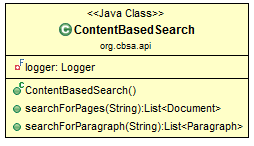
\includegraphics{class-dig-api}
\caption{Class Diagram - API}
\end{figure}

\begin{figure}[H]
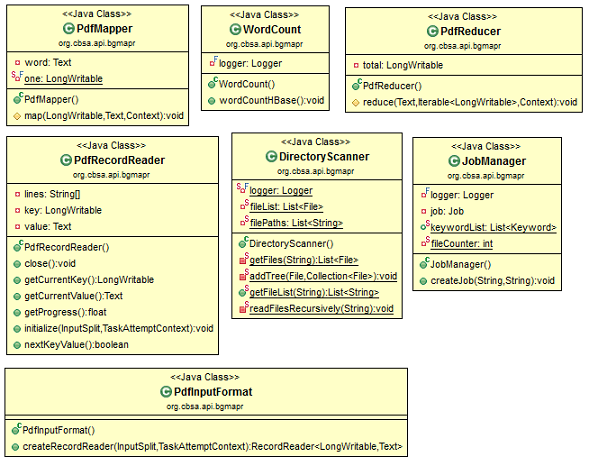
\includegraphics{class-dig-bgmapper}
\caption{Class Diagram - BGMapper}
\end{figure}

\begin{figure}[H]
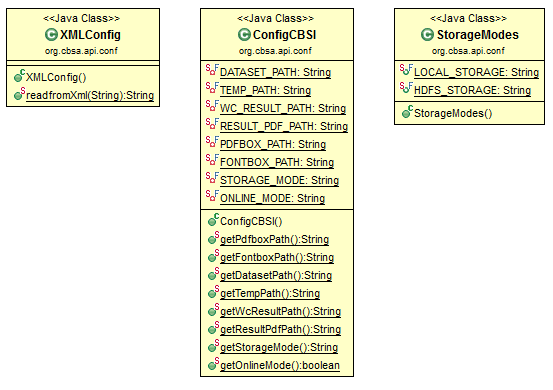
\includegraphics{class-dig-conf}
\caption{Class Diagram - Configuration}
\end{figure}

\begin{figure}[H]
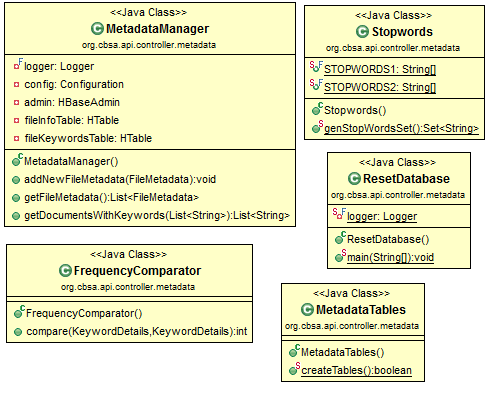
\includegraphics{class-dig-metadata}
\caption{Class Diagram - Metadata}
\end{figure}

\begin{figure}[H]
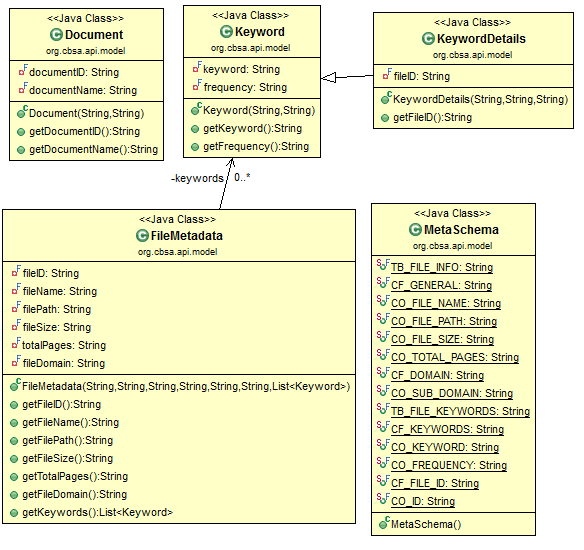
\includegraphics{class-dig-model}
\caption{Class Diagram - Model}
\end{figure}

\begin{figure}[H]
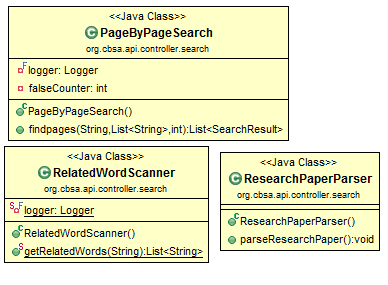
\includegraphics{class-dig-search}
\caption{Class Diagram - Search}
\end{figure}


% Chapter 8 :  Project Implementation

\chapter{Project Implementation}
\section{Introduction}
A software implementation method is a systematically structured approach to effectively integrate software based service or component into the workflow of an organizational structure or an individual end-user. A product software implementation method is a blueprint to get users and/or organizations running with a specific software product. The method is a set of rules and views to cope with the most common issues that occur when implementing a software product: business alignment from the organizational view and acceptance from the human view. The implementation of product software, as the final link in the deployment chain of software production, is in a financial perspective of a major issue. It is stated that the implementation of (product) software consumes up to 1/3 of the budget of a software purchase (more than hardware and software requirements together).

\section{Tools and Technologies Used}
 \subsection{Apache Hadoop}
 \begin{figure}[h]
 	\begin{center}
 		\fbox{
\includegraphics[width=100pt]{hadoop-logo}}
 	\end{center}
 	\caption{Hadoop logo}
 \end{figure} 
 The Apache Hadoop software library is a framework that allows for the distributed processing of large data sets across clusters of computers using simple programming models. It is designed to scale up from single servers to thousands of machines, each offering local computation and storage. Rather than rely on hardware to deliver high-availability, the library itself is designed to detect and handle failures at the application layer, so delivering a highly-available service on top of a cluster of computers, each of which may be prone to failures.

\subsection{Apache HBase}
 \begin{figure}[h]
 	\begin{center}
 		\fbox{
\includegraphics[width=100pt]{hbase-logo}}
 	\end{center}
 	\caption{HBase logo}
 \end{figure} 
HBase is a distributed column-oriented database built on top of the Hadoop file system. It is an open-source project and is horizontally scalable.

HBase is a data model that is similar to Google’s big table designed to provide quick random access to huge amounts of structured data. It leverages the fault tolerance provided by the Hadoop File System (HDFS).

It is a part of the Hadoop ecosystem that provides random real-time read/write access to data in the Hadoop File System.

One can store the data in HDFS either directly or through HBase. Data consumer reads/accesses the data in HDFS randomly using HBase. HBase sits on top of the Hadoop File System and provides read and write access.
 
 \subsection{Java Technology}
 
 Java is a general-purpose, concurrent, class-based, object-oriented computer programming language that is specifically designed to have as few implementation dependencies as possible. It is intended to let application developers ”write once, run anywhere” (WORA), meaning that code that runs on one platform does not need to be recompiled to run on another. Java applications are typically compiled to byte code (class file) that can run on any Java virtual machine (JVM) regardless of computer architecture. Java is, as of 2012, one of the most popular programming languages in use, particularly for client-server web applications, with a reported 10 million users. Java was originally developed by James Gosling at Sun Microsystems (which has since merged into Oracle Corporation) and released in 1995 as a core component of Sun Microsystems’ Java platform. The language derives much of its syntax from C and C++, but it has fewer low-level facilities than either of them. The original and reference implementation Java compilers, virtual machines, and class libraries were developed by Sun from 1991 and first released in 1995. As of May 2007, in compliance with the specifications of the Java Community Process, Sun relicensed most of its Java technologies under the GNU General Public License. Others have also developed alternative implementations of these Sun technologies, such as the GNU Compiler for Java and GNU Class path.
 \\
 Features Of Java are :  	
 \begin{enumerate}
 	\item Simple
 	\item Architecture neutral
 	\item Object oriented
 	\item Portable
 	\item Distributed	
 	\item High performance
 	\item Interpreted	
 	\item Multithreaded
 	\item Robust
 	\item Dynamic
 	\item Secure	x
 \end{enumerate}
 
 Java platform is the name for a bundle of related programs from Sun that allow for developing and running programs written in the Java programming language. The platform is not specific to any one processor or operating system, but rather an execution engine (called a virtual machine) and a compiler with a set of libraries that are implemented for various hardware and operating systems so that Java programs can run identically on allof them.

 
 \subsection{Eclipse}
 Eclipse is an open source community whose projects building tools and frameworks are used for creating general purpose application. The most popular usage of Eclipse is as a Java development environment .
 
 Eclipse is an open source community, whose projects are focused on building an open development platform comprised of extensible frameworks, tools and runtimes for building,deploying and managing software across the lifecycle. The Eclipse Foundation is a not-for-profit, member supported corporation that hosts the Eclipse projects  and helps cultivate both an open source community and an ecosystem of complementary products and services.
 The Eclipse Project was originally created by IBM in November 2001 and supported by a consortium of software vendors. The Eclipse Foundation was created in January 2004 as an independent not-for-profit corporation to act as the steward of the Eclipse community. The independent not-for-profit corporation was created to allow a vendor neutral and open, transparent community to be established around Eclipse. Today, the Eclipse community consists of individuals and organizations from a cross section of the software industry.

\section{Methodologies/Algorithm Details}

\begin{algorithm}[H]
\begin{enumerate}
\item Take Input Query from User
\item Use the Suffix Stripping Algorithm to remove English Suffixes like 'ed','ing',' ' 's ' to extract keywords
\item Match keywords with Documents' metadata present in Hbase and filter the documents to be searched.
\item Apply Searching Algorithm based on map-reduce operations like keyword count,positions.
\begin{itemize}
\item Open the PDF
\item Distribute the text using map operation.
\item combine the results with reduce operations.
\end{itemize} 
\item Sort the documents which are returned by Searching w.r.t keyword count and relevance.
\item Depending on API methods return the result with 
\begin{itemize}
\item Paragraph
\item Whole Page
\item Current and Previous Page
\end{itemize}
\end{enumerate}
\caption{Content Based Search Algorithm}
\end{algorithm}

\newpage

\begin{algorithm}[H]
\begin{enumerate}
\item Take the input pdf files from user
\item Check if corrupt
\item Upload the file into the Hadoop Distributed Filesystem
\item Run the Metadata Extracting Algorithm using the Map Reduce Engine.
\item Extract the Bibliography and Index Contents of each and every document (if present) and related keywords.
\item Store it in the HBase as metadata.
\item This metadata will be used by map reduce engine to search and retrieve data from relevant document inside HDFS using keyword relative custom partitioning.
\item Return the result to the search API
\item Stop
\end{enumerate}
 \caption{Meta-data Extraction Service Algorithm}
\end{algorithm}

% Chapter 9 :  Software Testing

\chapter{Software Testing}
\section{Type of Testing Used}

\subsection{Unit Testing : }
Unit testing refers to tests that verify the functionality of a specific section of code, usually at the function level. In an object-oriented environment, this is usually at the class level, and the minimal unit tests include the constructors and destructors. These types of tests are usually written by developers as they work on code (white-box style), to ensure that the specific functionis working as expected. One function might have multiple tests, to catch corner cases or other branches in the code. Unit testing alone cannot verify the functionality of a piece of software, but rather is used to assure that the building blocks the software uses work independently of each other. Unit testing is also called component testing.

\subsection{White Box Testing : }
White-box testing is a method of testing software that tests internal structures or workings of an application, as opposed to its functionality (i.e. black-box testing). In white-box testing an internal perspective of the system, as well as programming skills, are required and used to design test cases. The tester chooses inputs to exercise paths through the code and determine the appropriate outputs. This is analogous to testingnodes in a circuit testing. Using white box testing method,software engineer can derive test case that: Guarantee that all independent paths within module have been exercised at least once. Exercise all the logical decisions on their true or false sides. Execute all loops on the boundaries and within their operational bounds. Exercise internal structure to insure their validity. While white-box testing can be applied at the unit, integration and system levels of the software testing process, it is usually done at the unit level. It can test paths within a unit, paths between units during integration, and between subsystems during a system level test.

\subsection{Black Box Testing : }
Black-box testing is a method of software testing that tests the functionality of an application as opposed to its internal structures or workings (see white-box testing). Specific knowledge of the application’s code/internal structure and programming knowledge in general is not required. Test cases are built around specifications and requirements, i.e., what the application is supposed to do. It uses external descriptions of the software, including specifications, requirements, and design to derive test cases. These tests can be functional or non-functional, though usually functional. The test designer selects valid and invalid inputs and determines the correct output. There is no knowledge of the test object’s internal structure. Black box testing attempts to find error in following categories: Incorrect and missing function, Interface errors, Errors in data structures or External database accesses, Behaviour or performance error ,Initialization and termination.

\subsection{IntegrationTesting : }
The purpose of integration testing is to verify functional, performance, and reliability requirements placed on major design items. These ”design items”, i.e. assemblages (or groups of units), are exercised through their interfaces using Black box testing, success and error cases being simulated via appropriate parameter and data inputs. Simulated usage of shared data areas and inter-process communication is tested and individual subsystems are exercised through their input interface.

\subsection{RegressionTesting : }
Regression testing is any type of software testing that seeks to uncover new errors, or regressions, in existing functionality after changes have been made to the software, such as functional enhancements, patches or configuration changes. The intent of regression testing is to assure that a change, such as a bug fix, did not introduce new bugs. ”One of the main reasons for regression testing is that it’s often extremely difficult for a programmer to figure out how a change in one part of the software will echoin other parts of the software components. Common methods of regression testing include re-running previously run tests and checking whether program behaviour has changed and whether previously fixed faults have re-emerged. Regression testing can be used to test a system efficiently by systematically selecting the appropriate minimum set of tests needed to adequately cover a particular change.

\subsection{Functional Testing : }
Functional Testing It’s a type of GUI testing where functionality of an application is tested. Testing of all features and functions of system software, hardware, etc. To ensure requirements and specifications are met. Functionality testing of software is testing conducted on a complete, integrated system to evaluate the system’s compliance with its specified requirements. Functionality testing falls within the scope of black box testing, and as such, should require no knowledge of the inner design of the code or logic. Also the basic functional requirements of the system should be fulfilled and tested.

\section{Test Cases and Test Results}
\begin{figure}[h]
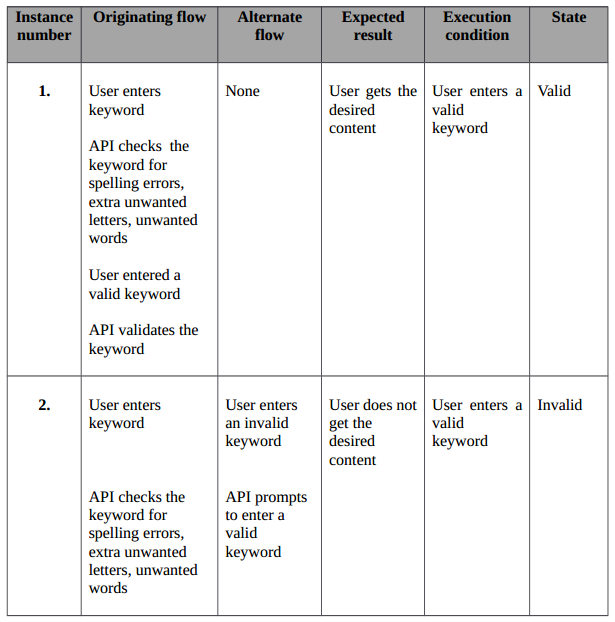
\includegraphics{test-case-1}
\caption{Test Case 1}
\end{figure}

\begin{figure}[h]
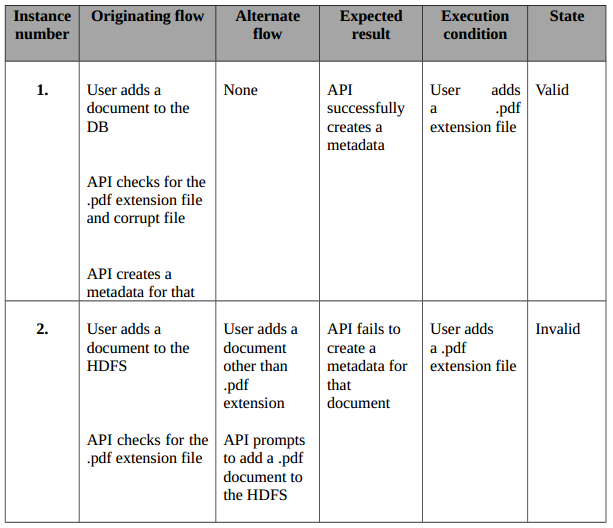
\includegraphics{test-case-2}
\caption{Test Case 1}
\end{figure}

\begin{figure}[h]
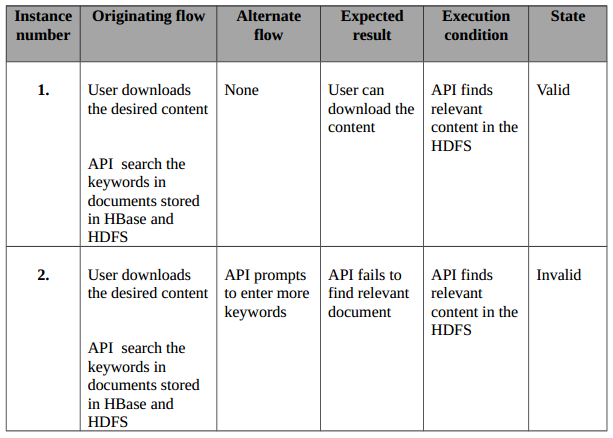
\includegraphics{test-case-3}
\caption{Test Case 1}
\end{figure}

This API had been tested for Technical e-books using page by page search algorithm and obtained relevant pages in single pdf file.\\\\
In above test case there were 10 different technical e-books was taken as dataset. Initially the metadata database had been maintained  in HBase consist of various relevant keywords in all the documents. These keywords used to filter the documents present in HDFS. In this case, 10 files were filtered to 2 files which was actually related to the test input.\\\\
After that content based search and retrieval performed on filtered documents using page by page search algorithm. Results were fairly accurate.


% Chapter 10 : Results
\chapter{Results}

\section{Screen shots}

\begin{figure}[H]
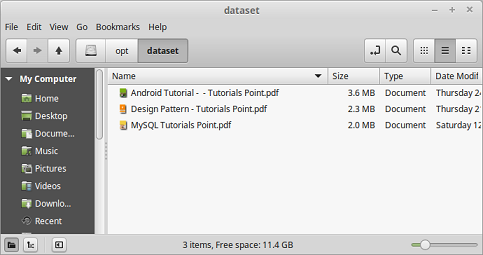
\includegraphics{results-dataset}
\caption{Results - Dataset}
\end{figure}

\begin{figure}[H]
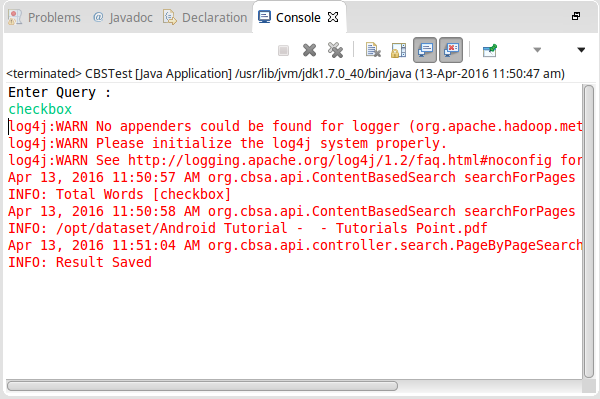
\includegraphics{results-console}
\caption{Results - Console}
\end{figure}

\begin{figure}[H]
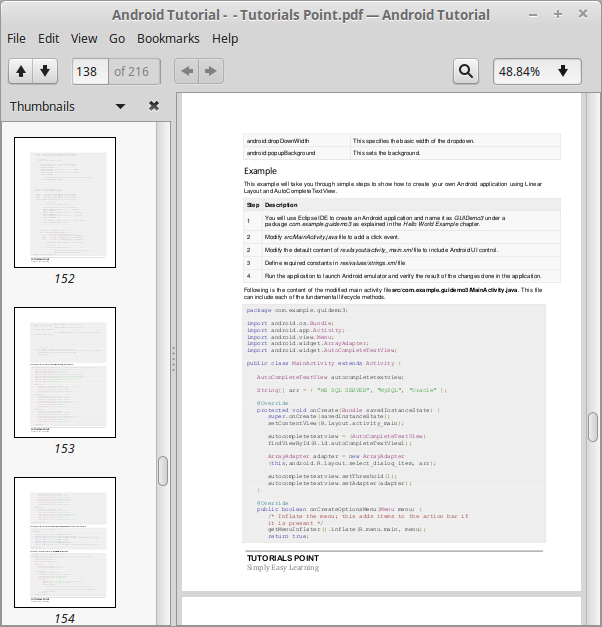
\includegraphics{results-before}
\caption{Results - Before}
\end{figure}

\begin{figure}[H]
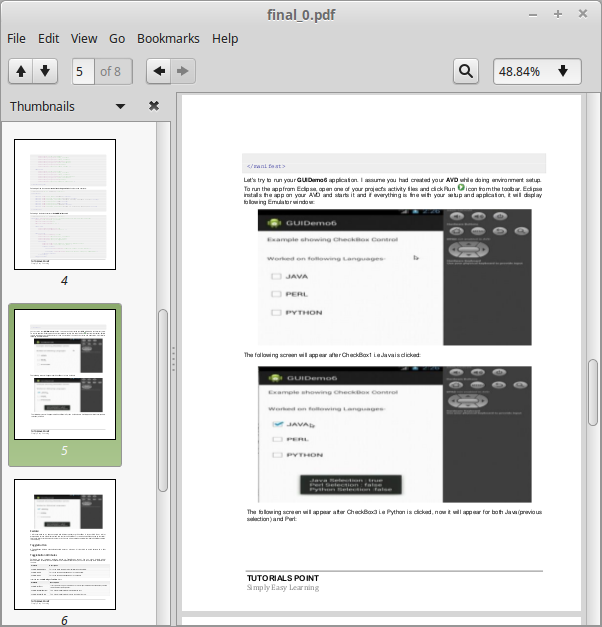
\includegraphics{results-after}
\caption{Results - After}
\end{figure}

\section{Outputs}
The dataset of pdf documents related to android, database, and design pattern technical books.\\\\
For Example: Input query is “Checkbox”
Then API will initially filter relevant documents from above dataset and then run content based search on those documents.\\\\
Here one document is filtered which is actually related to input query. The original size of document is large and has around 200 pages. \\\\
But after applying content based search on this filtered document output is generated in single pdf of relevant pages only. Result pdf is around 8 pages.


% Chapter 11 : Deployment And Maintainence
\chapter{Deployment and Maintenance}

Software deployment is all of the activities that make a software system available for use. The general deployment process consists of activities with possible transitions between them. These activities can occur at the producer site or at the consumer site or both. Because every software system is unique, the precise processes or procedures within each activity can hardly be defined. Therefore, ”deployment” should be interpreted as a general process that has to be customized according to specific requirements or characteristics. \\
We are deploying our application in hadoop cluster.

\section{Installation and un-installation}
\subsection{API Installation}
	\begin{enumerate}
	\item Download CBSA.tar.gz 
	\item Extract CBSA.tar.gz to /usr/local
	\item \$sudo tar -xvf CBSA.tar.gz -C /usr/local
	\item Open /usr/local/cbsa/etc/conf.xml
	\item Provide dataset\_path,  temp\_path, wc\_result\_path,  result\_pdf\_path, storage\_mode, online\_mode
	\end{enumerate}
\section{User help}
\noindent\textbf{Q) How to install this API?}\\
The first step is to configure this Hadoop API using etc/conf.xml for all the input files and the output to be generated and the various settings like hdfs file system and online/offline modes.And then the jar can be added either using the external jar referencing in the IDE like eclipse/netbeans or adding using mvnrepository.\\\\

\noindent\textbf{Q) How to Use this Api as a developer?}\\
The first step is to extract the metadata of the documents using the WordCount Class so that the metadata gets indexed in the HBase database and then using the seach and retrieval API for extracting the Contents of PDF.\\\\

\noindent\textbf{Q) What background is needed to Use this Api?}\\
->The Only background required for the user of this API is basic JAVA programming and basic depth in Hadoop programming.\\\\

\noindent\textbf{Q) How to contribute to this project?}\\
This project is an opensourced at https://github.com/hadoop-addon-for-advanced-context-based-search-and-retrieval.So the enthusiasts can clone the project and send their pull requests following certain open source contribution standards.Also the pull requests to be added have to be clearly documented and tested.\\\\

\noindent\textbf{Q) What are the areas of contribution?}\\
There are several areas for contribution like creating API for parsing files for processing PDF files in HDFS,extracting metadata from other file formats like ePub,mobi,doc,docx by creating custom recordreaders,internationalization for indexing other language files.\\\\

\noindent\textbf{Q) How can I extend this API to other type of file formats?}\\
->By extending the logic of RecordReader to other formats like epubs and docx as well as creating a mechanism to support language other than English this API van be further extended.\\\\

\noindent\textbf{Q) What are the license issues for this API?}\\
This API uses several Apache components like Commons,Hadoop,PdfBox and hence this API shall support Apache License for OpenSource.\\\\

\noindent\textbf{Q) How to use this API's offline mode?}\\
By changing the conf.xml to offline mode we can enable online dictionary to support meaningful searches which can be of use in fiction and non-fictional books.


\chapter{Summary and Conclusion}
\section{Summary}
Unstructured data like doc, pdf, accdb is lengthy to search and filter for desired information. We need to go through every file manually for finding information. It is very time consuming and frustrating. It doesn’t need to be done this way if we can use high computing power to achieve much faster content retrieval. This addon will be able to provide APIs for different search results and able to download full file, part of files which are actually related to that topic. 

\section{Conclusion}
Thus we can use this API in Hadoop to reduce manual efforts and bring advance content based search and retrieval

\section{Future Scope}
Extending our API further to read scanned text copies and retrieve the data from them would solve further advanced issues. This API again can be extended further to work with Image processing so that it may find a relevant information from the digital images for the end- users.\\\\
We can also extend the API of CBSA to work on research paper by implementing a reseach paper parser using the Apache PDFBox so that the content can be extended for Research paper search and retrieval which typically has a two column format of PDF files.\\\\
We can also extend the API to work on multiple file formats like ePUB3,mobi,.odt,.docx by implementing the required RecordReader for the Hadoop Mappers to support such formats.\\\\
This API can be extended for content based searching and retriving from paragraph.


% Annexure
\begin{appendices}

% Annexure A :  References
\begin{thebibliography}{7}

\bibitem {R1} Parul Gupta, Dr. A.K. Sharma, “Content based Indexing in Search Engines using Ontology ”,2010

\bibitem {R2} Lars George, ”HBase: The Definitive Guide”, 1st edition, O’Reilly Media, September 2011,   ISBN 9781449396107

\bibitem {R3} Tom White, ”Hadoop: The Definitive Guide”, 1st edition, O’Reilly Media, June 2009, ISBN 9780596521974

\bibitem {R4} Apache Hadoop HDFS homepage http://hadoop.apache.org/hdfs/

\bibitem {R5} MehulNalinVora ,”Hadoop-HBase for Large-Scale Data”,InnovationLabs,PERC,ICCNT Conference

\bibitem {R6} YijunBei,ZhenLin,ChenZhao,Xiaojun Zhu ,”HBase System-based Distributed Framework for Searching Large Graph Databases”,ICCNT Conference

\bibitem {R7} SeemaMaitrey,C.K.”Handling Big Data Efficiently by using Map Reduce Technique”,ICCICT

\bibitem {R8} Maitrey S, Jha. An Integrated Approach for CURE Clustering using Map-Reduce Technique. In Proceedings of Elsevier,ISBN 978-81- 910691-6-3,2 nd August 2013


\end{thebibliography}

% Annexure B

\chapter{Laboratory assignments on Project Analysis of Algorithmic Design}


\section{ASSIGNMENT NO 1}

\textbf{Objective :} \\

To develop the problem under consideration and justify feasibilty using concepts of knowledge canvas and IDEA Matrix.

\textbf{Feasibility Study : } \\
Feasibility study is an evaluation and analysis of the potential of a proposed project which is based on extensive investigation and research to support the process of decision making.
\\
Feasibility study has been done on following parameters:--
\begin{itemize}
\item Technical feasibility.
\item Economic feasibility.
\item Operational feasibility.
\end{itemize}

\textbf{IDEA Matrix : }

  \begin{center}
	\begin{figure}[H]
		\centering
		\fbox{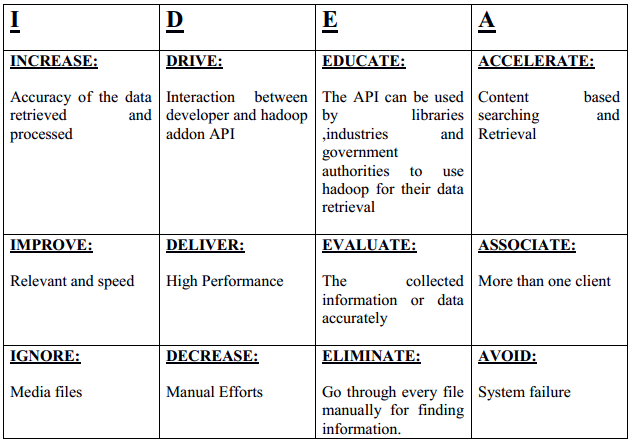
\includegraphics[width=\textwidth]{idea_matrix}}
	  \caption{IDEA Matrix}
	  \label{fig:arch-dig}
	\end{figure}
\end{center} 

\section{ASSIGNMENT NO 2}

\textbf{Objective :} \\

\textbf{P - Problem :} \\
A problem is assigned to the P (polynomial time) class if there exists at least one algorithm to solve that problem, such that the number of steps of the algorithm is bounded by a polynomial in O(n), where n is the size of the input. \\


\textbf{NP - Problem :} \\
A problem is assigned to the NP (nondeterministic polynomial time) class if it is solvable in polynomial time by a non deterministic Turing machine. \\

\textbf{NP - Hard :} \\
A problem is said to be NP-hard if an algorithm for solving it can be translated into one for solving any other NP-problem. It is much easier to show that a problem is NP than to show that it is NP-hard. \\

\textbf{NP - Complete :} \\
A problem which is both NP and NP-hard is called an NP-complete problem. 
\\

On the basis of the above definitions, our problem statement is solvable in polynomial time by deterministic Turing machine hence it   is said to be P-Problem. \\

\noindent \textbf{Mathematical Model for the project :} \\
S = \{s,e,x,y,DD,NDD,Mem-shared\} \\\\
s = start state : Taking input from the user as search query \\
e = End State : return the output to the user in the form text based content \\\\
x = Input : Search Query \\
y = Output : Text Based Result \\\\
DD = Deterministic Data \\
1) Number of PDF Files \\
2) Keyword Tokenisation and Filteration \\
3) Number of DataNodes 
4) Search Progress 
5) Number of Results Obtained \\\\
NDD = Non Deterministic Data \\
1) Failure of Cluster Nodes \\
2) Communication Failure  \\\\
Mem-Shared = Storage Space 
1) HDFS will be distributed among a number of nodes in Hadoop Cluster and will share common FileSystem which will be managed by Hadoop \\

% Annexure C

\chapter{Laboratory assignments on Project Quality and Reliability Testing of Project Design}

\section{ASSIGNMENT NO 3}

\textbf{Objective :} \\
Use of Divide and Conquer strategies to exploit distributes/parallel/ concurrent processing of the above to identify objects, morphisms, overloading in functions (if any) and functional relations and any other dependencies (as per requirements). \\

\textbf{Divide And Conquer : } \\
Divide and Conquer is an algorithm design paradigm based on multi branched recursion. A typical Divide and Conquer algorithm solves a problem using following three steps. \\

\begin{itemize}
\item \textbf{Divide :} Break the given problem into sub-problems of same type.
\item \textbf{Conquer :} Recursively solve these sub-problems.	
\item \textbf{Combine :} Appropriately combine the solutions to the sub-problems. The solutions to the sub-problems are combined to produce a solution to the given problem.
\end{itemize}

\textbf{Demonstration : } \\

\begin{itemize}
\item \textbf{Divide :} Divide the search by mapping the input by using mappers of Map Reduce.
\item \textbf{Conquer :} Reduce the number of search by aggregation.
\item \textbf{Combine :} Combine the relevant searches as per the keywords entered.
\end{itemize}

\pagebreak
\textbf{Divide And Conquer Diagram : }

 \begin{center}
	\begin{figure}[!htbp]
		\centering
		\fbox{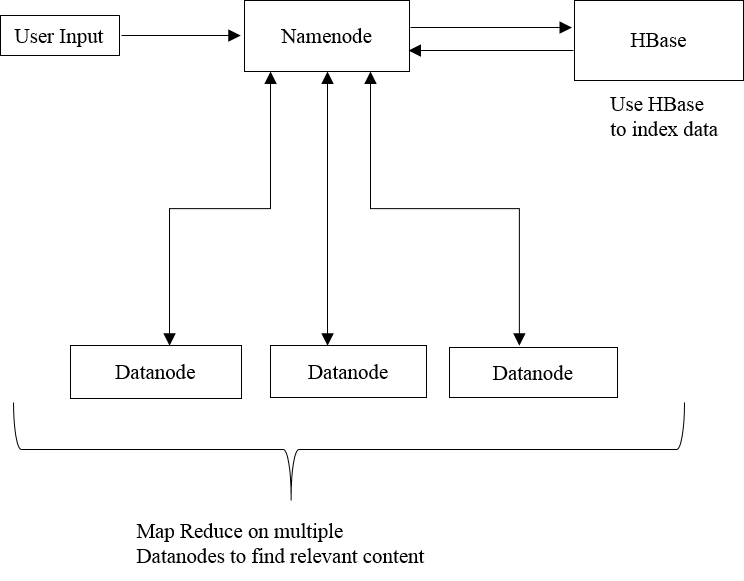
\includegraphics[width=\textwidth]{architecture_design}}
	  \caption{Multi Cluster Diagram}
	  \label{fig:arch-dig}
	\end{figure}
\end{center} 

\pagebreak

\section{ASSIGNMENT NO 4}

\textbf{Objective : } \\
Use of the above to draw functional dependency graphs and relevant software modelling methods , techniques including UML diagrams or other necessities using appropriate tools. \\

\textbf{Use Case Diagram : }

\begin{center}
	\begin{figure}[H]
		\centering
		\fbox{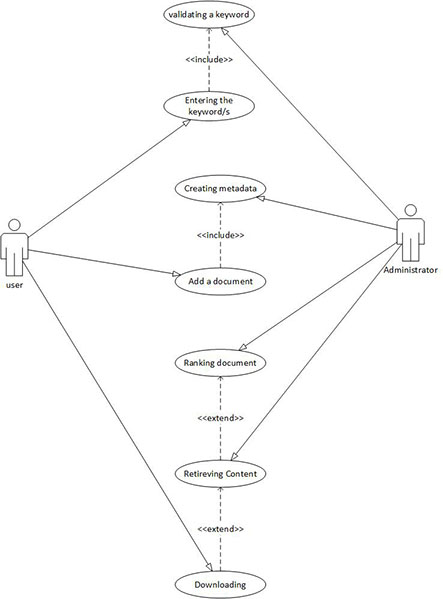
\includegraphics[width=230pt]{use_case_diagram}}
	  \caption{Use Case Diagram}
	  \label{fig:state-dig}
	\end{figure}
\end{center} 

\pagebreak
\textbf{Activity Diagram : }

\begin{center}
	\begin{figure}[H]
		\centering
		\fbox{
\includegraphics[width=230pt]{activity_diagram}}
	  \caption{Activity Diagram}
	  \label{fig:state-dig}
	\end{figure}
\end{center} 


\pagebreak
\section{ASSIGNMENT NO 5}

\textbf{Objective : }Testing of project problem statement using generated test data (using mathematical models, GUI, Function testing principles, if any) selection and appropriate use of testing tools, testing of UML diagram’s reliability  \\

\noindent \textbf{Mathematical Model for the project :} \\
S = \{s,e,x,y,DD,NDD,Mem-shared\} \\\\
s = start state : Taking input from the user as search query \\
e = End State : return the output to the user in the form text based content \\\\
x = Input : Search Query \\
y = Output : Text Based Result \\\\
DD = Deterministic Data \\
1) Number of PDF Files \\
2) Keyword Tokenisation and Filteration \\
3) Number of DataNodes 
4) Search Progress 
5) Number of Results Obtained \\\\
NDD = Non Deterministic Data \\
1) Failure of Cluster Nodes \\
2) Communication Failure  \\\\
Mem-Shared = Storage Space 
1) HDFS will be distributed among a number of nodes in Hadoop Cluster and will share common FileSystem which will be managed by Hadoop \\

\noindent \textbf{Test cases :}

\begin{center}
	\begin{figure}[H]
		\centering
		\fbox{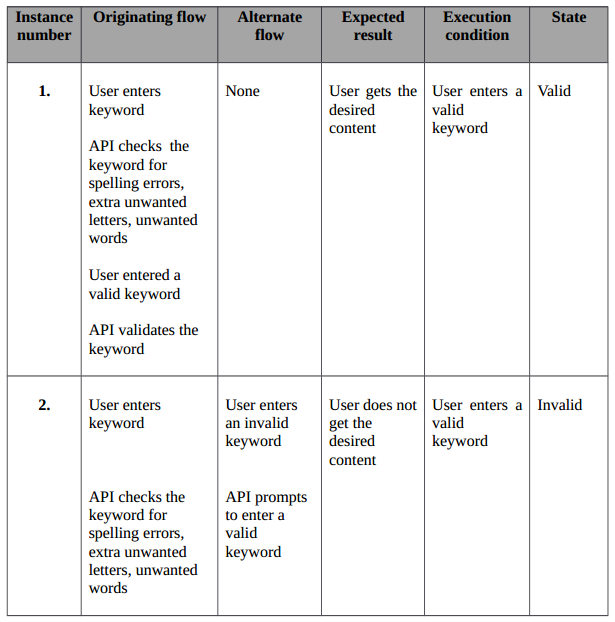
\includegraphics[width=230pt]{test-case-1}}
	  \caption{Test Case 1}
	  \label{fig:state-dig}
	\end{figure}
\end{center} 

\begin{center}
	\begin{figure}[H]
		\centering
		\fbox{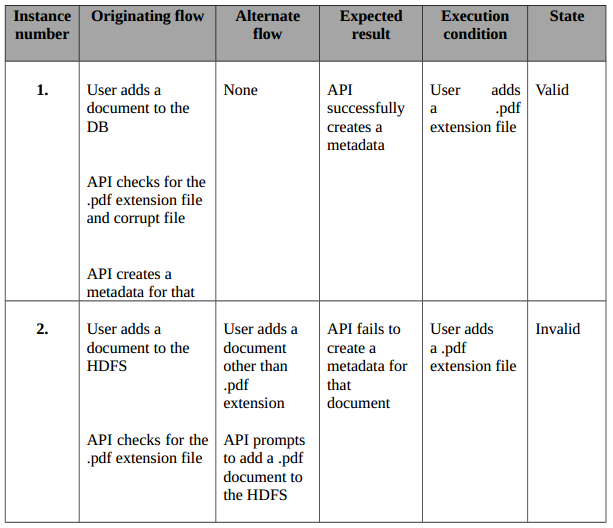
\includegraphics[width=230pt]{test-case-2}}
	  \caption{Test Case 2}
	  \label{fig:state-dig}
	\end{figure}
\end{center} 

\begin{center}
	\begin{figure}[H]
		\centering
		\fbox{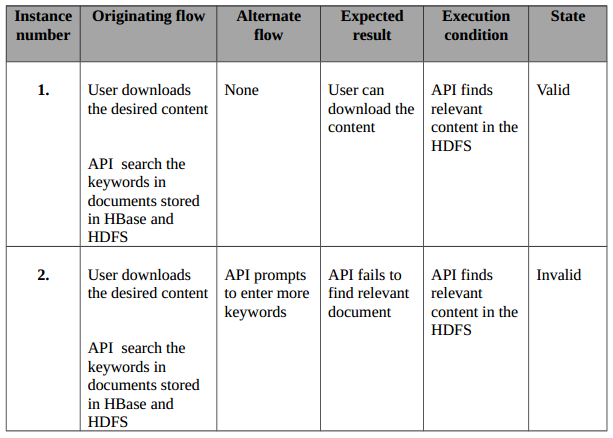
\includegraphics[width=230pt]{test-case-3}}
	  \caption{Test Case 3}
	  \label{fig:state-dig}
	\end{figure}
\end{center} 

\chapter{Project Planner}
\label{app:plan}

Major Tasks in the Project stages are:
\begin{itemize}
\item Create distributed system with Hadoop namenodes and datanodes
\item Develop API methods for extracting keywords from input query
\item Test API methods for finding keywords from input query
\item Develop API methods to perform keyword search on HDFS data using Map Reduce operations
\item Test API methods to perform keyword search on HDFS data using Map Reduce operations
\item Design database schema for indexing each and every document in HDFS
\item Schema validation for HBase indexing database
\item Develop background service for indexing newly added data to HBase database automatically
\item Test background service for indexing newly added data to HBase database is working automatically or not
\item Integrating all modules
\item Integration testing
\end{itemize}

\begin{center}
	\begin{figure}[!htbp]
		\centering
		\fbox{
\includegraphics[width=\textwidth]{task_network}}
	  \caption{Project Planning Chart 1}
	  \label{fig:usecase}
	\end{figure}
\end{center} 

\begin{center}
	\begin{figure}[!htbp]
		\centering
		\fbox{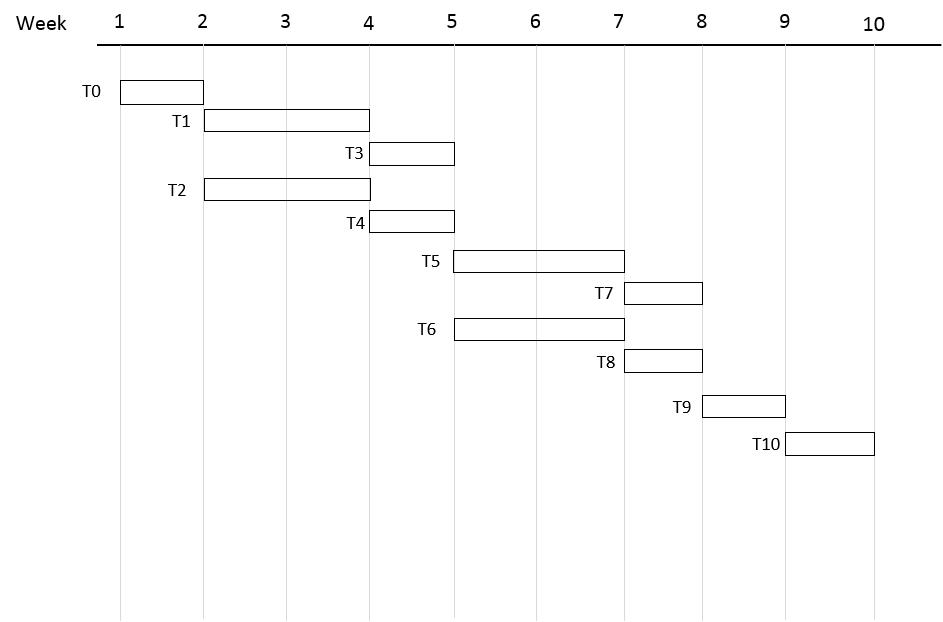
\includegraphics[width=\textwidth]{timeline_chart}}
	  \caption{Project Planning Chart 2}
	  \label{fig:usecase}
	\end{figure}
\end{center} 

\chapter{Reviewers Comments of Paper Submitted}

\begin{enumerate}
\item \textbf{Paper Title } : Hadoop add-on API for Advanced Content Based Search \& Retrieval 
\item \textbf{Name of the Conference/Journal where paper submitted } : IOSR - International Organization of Scientific Research
\item \textbf{Paper accepted/rejected } : Accepted
\item \textbf{Review comments by reviewer} : The independent review upon your research article titled "Hadoop add-on API for Advanced Content Based Search \& Retrieval" has been provided by the concerned referees. The referees have suggested Accepted your paper in IOSR Journals.
	\begin{enumerate}
		\item Quality of Manuscript is good.
		\item Consolidated Decision: Accepted for publication 
	\end{enumerate}
	
\end{enumerate}

\begin{enumerate}
\item \textbf{Paper Title } : Content Based Search Add-on API Implemented for Hadoop Ecosystem
\item \textbf{Name of the Conference/Journal where paper submitted } : -- pending
\item \textbf{Paper accepted/rejected } : -- pending
\item \textbf{Review comments by reviewer} : -- pending
	
\end{enumerate}


\chapter{Plagiarism Report}
\begin{center}
	\begin{figure}[!htbp]
		\centering
		\fbox{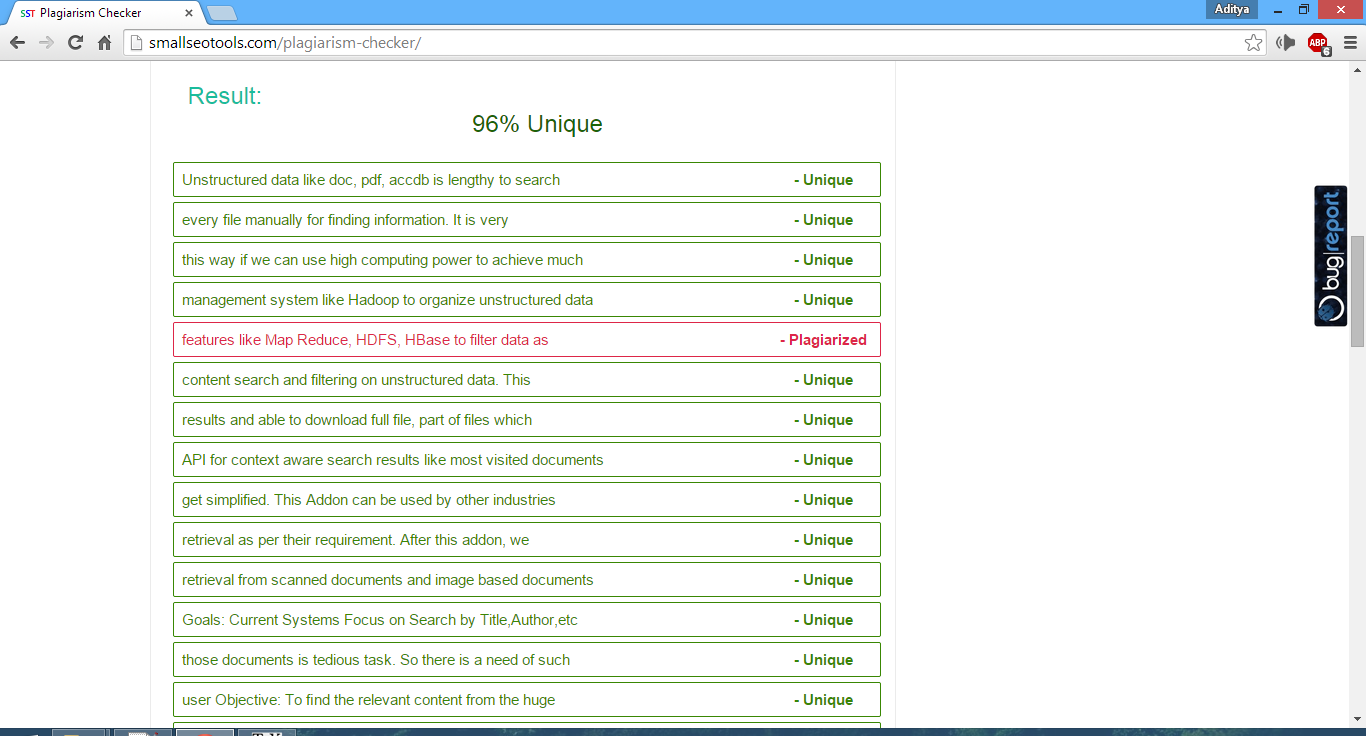
\includegraphics[width=\textwidth]{plagiarism_report}}
	  \caption{Plagiarism Report}
	  \label{fig:usecase}
	\end{figure}
\end{center}  


\chapter{ Term-II Project Laboratory Assignments}

\section{ASSIGNMENT NO 1}

\textbf{Aim :} \\

Review of design and necessary corrective actions taking into consideration the feedback report of Term I assessment, and other competitions/conferences participated like IIT, Central Universities University Conferences or equivalent centre of excellence etc.
\\

\noindent \textbf{Publications :} \\

\begin{enumerate}
\item \textbf{Paper Title } : Hadoop add-on API for Advanced Content Based Search \& Retrieval 
\item \textbf{Name of the Conference/Journal where paper submitted } : IOSR - International Organization of Scientific Research
\item \textbf{Paper accepted/rejected } : Accepted
\item \textbf{Review comments by reviewer} : The independent review upon your research article titled "Hadoop add-on API for Advanced Content Based Search \& Retrieval" has been provided by the concerned referees. The referees have suggested Accepted your paper in IOSR Journals.
	\begin{enumerate}
		\item Quality of Manuscript is good.
		\item Consolidated Decision: Accepted for publication 
	\end{enumerate}
	
\end{enumerate}

\pagebreak

\section{ASSIGNMENT NO 2: }

\textbf{Aim} : Project Workstation Selection, Installations Along With Setup and installation Report Preparations \\\\

\noindent \textbf{Project WorkStation Selection : } 
\begin{itemize}
\item Our project is based on Apache Hadoop, based on Hbase. 
\item Our API requires minimum 100 MB space as it contains core components for content based retrieval.
\item 4 GB Primary Memory / RAM
\item Intel i3/i5/i7 64bit or AMD Processors
\end{itemize}


\noindent \textbf{Installation Steps : }
\begin{itemize}
\item Any Open Source Linux Distribution.(Ubuntu Server version 14.04.2 Pre-ferred)
\item OPENSSH installed on each machine with public key of each node in Authorized keys directory along with the local host.
\item We need to install the following tools:
	\begin{itemize}
		\item Eclipse IDE
		\item Hadoop Eclipse Plugin
		\item Java 1.7
		\item Hadoop Java Libraries. 
	\end{itemize}
\end{itemize}


\noindent \textbf{Installations} :

\noindent The installation steps are as follows:\\

\noindent \textbf{Step One: Hadoop Installation} \\\\
Unpack the downloaded Hadoop distribution. In the distribution,\\
edit the file etc/hadoop/hadoop-env.sh to define some parameters as follows: \\

\noindent set to the root of your Java installation \\
  export JAVA\_HOME=/usr/java/latest \\

\noindent Assuming your installation directory is /usr/local/hadoop \\
  export HADOOP\_PREFIX=/usr/local/hadoop \\

\noindent Try the following command: \\

  \$ bin/hadoop \\


\noindent Refer configuration files in this dir to configure your hadoop and yarn \\
  
\noindent Format the filesystem: \\

  \$ bin/hdfs namenode -format \\

\noindent Start NameNode daemon and DataNode daemon: \\

  \$ sbin/start-dfs.sh \\

\noindent The hadoop daemon log output is written to the \$HADOOP\_LOG\_DIR directory (defaults to \$HADOOP\_HOME/logs).
Browse the web interface for the NameNode; by default it is available at: \\

    NameNode - http://localhost:50070/ \\

\noindent Make the HDFS directories required to execute MapReduce jobs: \\

  \$ bin/hdfs dfs -mkdir /user \\
  \$ bin/hdfs dfs -mkdir /user/username \\

\noindent Copy the input files into the distributed filesystem: \\

  \$ bin/hdfs dfs -put etc/hadoop input \\

\noindent Run some of the examples provided: \\

  \$ bin/hadoop jar share/hadoop/mapreduce/hadoop-mapreduce-examples-2.6.0.jar grep input output 'dfs[a-z.]+' \\

\noindent Examine the output files: \\

\noindent Copy the output files from the distributed filesystem to the local filesystem and examine them: \\

  \$ bin/hdfs dfs -get output output \\
  \$ cat output/*  \\
  
\noindent To start yarn \\
  \$\$HADOOP\_HOME/sbin/start-yarn.sh \\
  
  
\noindent To stop dfs and yarn \\
  \$\$HADOOP\_HOME/sbin/stop-dfs.sh \\
\$\$HADOOP\_HOME/sbin/stop-yarn.sh \\


\noindent \textbf{Step Two: Hbase Installation} \\\\

\$sudo tar -xvf hbase-1.1.2-bin.tar.gz -C /usr/local \\
\$sudo mv /usr/local/hbase-1.1.2 /usr/local/hbase \\
\$sudo chown aditya:aditya -R /usr/local/hbase \\ \\

refer configuration files to setup hbase for standalone and pseudo distributed mode


\pagebreak

\section{ASSIGNMENT NO 3}

\textbf{Aim : }Programming of the project functions, interfaces and GUI (if any) as per 1 st Term term-work submission using corrective actions recommended in Term-I assessment of Term-work.\\

\noindent \textbf{Project modules are } : \\
1.	Background map reduce module for keyword extraction \\
2.	Configuration module \\
3.	Metadata manager module \\
4.	Search module for page by page search \\
5.	Models for keyword schema and file metadata \\

\noindent \textbf{1.	Background map reduce module for keyword extraction} \\
A Map Reduce program is composed of a Map() procedure(method) that performs filtering and sorting and a Reduce() method that performs a summary operation. The Map Reduce System run the various tasks in parallel, managing all communications and data transfers between the various parts of the system.\\

\begin{itemize}
\item Take Input Query from User 
\item Use the Suffix Stripping Algorithm to remove English Suffixes like ’ed’,’ing’,’ ’ ’s ’ to extract keywords 
\item Match keywords with Documents’ metadata present in Hbase and filter the documents to be searched. 
\item Apply Searching Algorithm based on map-reduce operations like keyword count, positions. 
	\begin{itemize}
		\item Open the PDF 
		\item Distribute the text using map operation. 	
		\item Combine the results with reduce operations. 
	\end{itemize}
\item Sort the documents which are returned by Searching w.r.t keyword count and relevance. 
\end{itemize}



\noindent \textbf{2.	Configuration module} :  \\
Whenever the content based API is initiated it checks for some basic configuration like where is the dataset, where are libraries, version of the libraries, temporary files path, where should the result output be stored, mode of dataset storage like local fs/hdfs  etc.\\


\noindent \textbf{3.	Metadata manager module } : \\
Searching and retrieving information from data inside HDFS. Hadoop Map Reduce operations will be used to perform key value pair generation and depend upon result information is searched. \\

\noindent a) Here, data is documents in PDF (Portable Document Format) format. These documents are stored on HDFS Hadoop Distributed File System. These documents are considered as raw data. These documents can have properties like 

\begin{itemize}
\item Name Size Date 
\item Author 
\end{itemize}

\noindent b)	Document meta data is also maintain in HBase distributed database. It has attributes like 
\begin{itemize}
\item Content Keywords
\item Index Keyword 
\item Document Keywords 
\end{itemize}

\noindent \textbf{4.	Search module for page by page search} : \\
This metadata will be used by map reduce engine to search and retrieve data from relevant document inside HDFS using keyword relative custom partitioning. And finally
Return the result to the search API .

\noindent \textbf{5.	Models for keyword schema and file metadata} : \\
Models for keyword schema consist of field KeywordId which makes algorithm to provide quick searching. After that each document under document scanner provides file id. When Hbase is queried for keyword using this indexing searching is easy.
File Meta data is also maintained in HBase distributed database. It has attributes like Content Keywords, Index Keyword and Document Keywords.



\pagebreak

\section{ASSIGNMENT NO 4}

\textbf{Aim : } Test tool selection and testing of various test cases for the project performed and generate various testing result charts, graphs etc. including reliability testing. \\

\noindent \textbf{Main Testing : }

\begin{center}
	\begin{figure}[!htbp]
		\centering
		\fbox{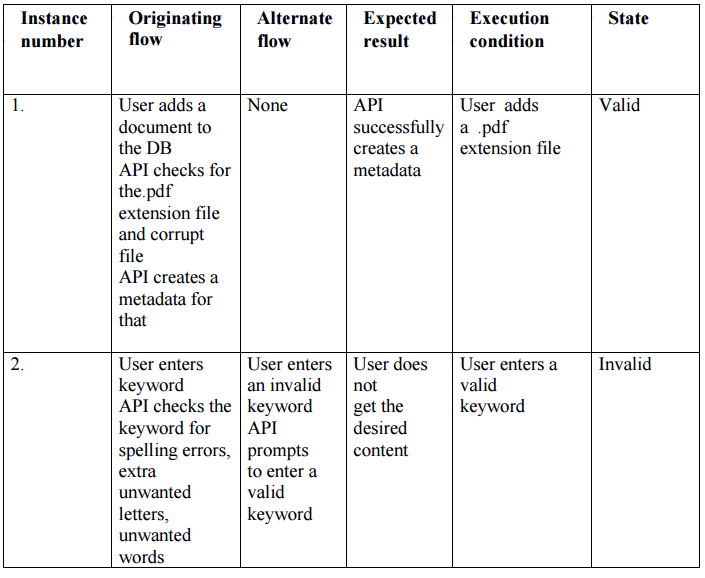
\includegraphics[width=\textwidth]{assignment-test-1}}
	  \caption{Assignment - Test Case 1}
	  \label{fig:usecase}
	\end{figure}
\end{center}  

\begin{center}
	\begin{figure}[!htbp]
		\centering
		\fbox{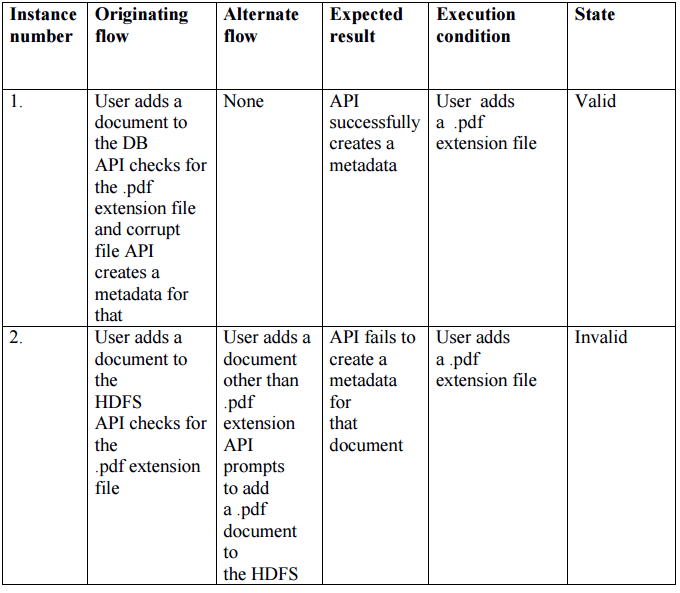
\includegraphics[width=\textwidth]{assignment-test-2}}
	  \caption{Assignment - Test Case 2}
	  \label{fig:usecase}
	\end{figure}
\end{center}  

\begin{center}
	\begin{figure}[!htbp]
		\centering
		\fbox{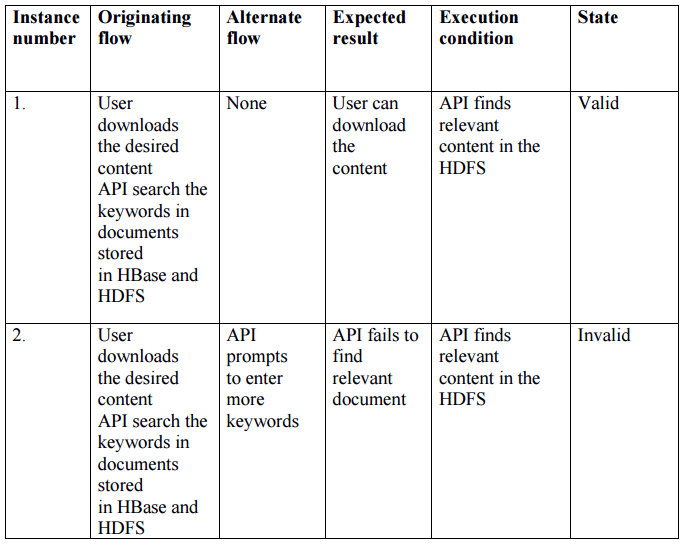
\includegraphics[width=\textwidth]{assignment-test-3}}
	  \caption{Assignment - Test Case 3}
	  \label{fig:usecase}
	\end{figure}
\end{center}  

\chapter{Information of Project Group Members}


\begin{enumerate}
	\item Name : Kshama Jain  \hspace{90 mm}
	%\includegraphics[width=60pt]{photo.jpg}
	\item Date of Birth : 22nd March 1995
	\item Gender : Female
	\item Permanent Address : Mahavir Marg, Paras Medical, Lane No - 3, Kusumba, Dist. Pune  
	\item E-Mail : jain.kshama9@gmail.com
	\item Mobile/Contact No. : 9405823495
	\item Placement Details : KPIT Technologies
\end{enumerate}
\pagebreak

\begin{enumerate}
	\item Name : Aditya Kamble  \hspace{90 mm}
	%\includegraphics[width=60pt]{photo.jpg}
	\item Date of Birth : 2nd Jan 1995
	\item Gender : Male
	\item Permanent Address : Plot No 29, Sadgurunagar, Near Nikam Hospital, Talegaon Dabhade, Taluka - Maval, Dist. Pune
	\item E-Mail : adityakamble49@gmail.com
	\item Mobile/Contact No. : 9960255708
	\item Placement Details : Xoriant Solutions Pvt. Ltd.
\end{enumerate}
\pagebreak

\begin{enumerate}
	\item Name : Rahul Rao  \hspace{90 mm}
	%\includegraphics[width=60pt]{photo.jpg}
	\item Date of Birth : 6th Jun 1994
	\item Gender : Male
	\item Permanent Address : Plot No 454/3, Sector 27/A Piyusha Apartments, Pradhikaran Nigdi Pune-411044
	\item E-Mail : rahulraopune@gmail.com
	\item Mobile/Contact No. : 7709008855
	\item Placement Details : Mercedes Benz Research and Development, Bengaluru
\end{enumerate}
\pagebreak

\begin{enumerate}
	\item Name : Siddhesh Palande  \hspace{90 mm}
	%\includegraphics[width=60pt]{photo.jpg}
	\item Date of Birth : 1st August 1994
	\item Gender : Male
	\item Permanent Address : H.A. Colony, Pimpri, Pune 411018
	\item E-Mail : sidpalande@gmail.com
	\item Mobile/Contact No. : 9657327798
	\item Placement Details : NTT Data
\end{enumerate}
\pagebreak


\end{appendices}
\end{document}
